\documentclass[english, 10pt, letterpaper]{article}
\usepackage[letterpaper, margin=0.8in]{geometry}
\usepackage[utf8]{inputenc}

\title{\emph{KRAS} allele-specific genetic interactions}
\author{
    Joshua Cook\textsuperscript{1,2, 7},
    Giorgio Melloni\textsuperscript{3, 7}, 
    Doga Gulhan\textsuperscript{3}, 
    Peter J. Park\textsuperscript{3,4{*}}, 
    Kevin M. Haigis\textsuperscript{1,2,5,6{*}}
}

\usepackage[T1]{fontenc}
\usepackage{babel}
\usepackage{amsmath}
\usepackage{amssymb}
\usepackage{graphicx}
\usepackage{fancyhdr}
\pagestyle{fancy}
\fancyhf{}
\renewcommand{\headrulewidth}{0pt}
\setlength{\headheight}{0pt}

% Supplementary figure numbering.
\newcommand{\beginsupplement}{%
        \setcounter{table}{0}
        \renewcommand{\thetable}{\arabic{table}}%
        \setcounter{figure}{0}
        \renewcommand{\thefigure}{\arabic{figure}}%
    }

% Single spaces after periods.
\frenchspacing

% Page numbering.
\pagenumbering{arabic}
\rfoot{\thepage}

% Font to Helvetica.
\usepackage{helvet}
\renewcommand{\familydefault}{\sfdefault}

% Specific command for the KRAS gene.
\newcommand{\KRAS}{\emph{KRAS}}
% Specific command for the KRAS protein.
\newcommand{\kras}{KRas}

\begin{document}

%%TC:ignore

\maketitle

\thispagestyle{fancy}

1. Department of Cancer Biology, Dana Farber Cancer Institute, Boston, Massachusetts.
2. Department of Medicine, Harvard Medical School, Boston, Massachusetts.
3. Department of Medical Informatics, Harvard Medical School, Boston, Massachusetts, USA.
4. Ludwig Center at Harvard, Boston, MA 02115, USA.
5. Broad Institute, Cambridge, Massachusetts, USA.
6. Harvard Digestive Disease Center, Harvard Medical School, Boston, Massachusetts.
7. These authors contributed equally.

{*}corresponding author(s):
\newline{} \hspace*{1cm} Kevin M. Haigis (khaigis@bidmc.harvard.edu)
\newline{} \hspace*{1cm} Peter J. Park (peter\_park@hms.harvard.edu)

\begin{abstract}
% Keep within 100-150 words.
Mutational activation of the \KRAS{} oncogene promotes initiation and/or progression of cancer in a variety of tissues.
Though the mutant variants seemingly exert similar biological outputs, the biochemical properties and downstream signaling  of each is distinct and highly context-dependent.
As such, the genetic interactions associated with \KRAS{} mutants are likely to vary according to the specific allele and the tissue-of-origin of the cancer.
To explore this concept, 13,492 samples were collated from four tumor types with the highest frequency of mutation in \KRAS{}: colorectal adenocarcinoma, lung adenocarcinoma, multiple myeloma, and pancreatic adenocarcinoma.
Each cancer had a distinct spectrum of \KRAS{} activating mutations that could not be predicted by the prevalence of known mutagenic mechanisms.
Moreover, each allele was associated with a distinct comutation network that was also tissue-specific.
Analyzing genetic dependencies highlighted cellular functions and individual genes that were or were not required for tumors with specific \KRAS{} alleles.
Overall, this analysis demonstrates that the \KRAS{} alleles have distinct genetic interactions likely linked to their biological differences.
\end{abstract}

%%TC:endignore

\section*{}

Sitting at a critical signaling junction between extracellular growth receptors and pro-growth pathways, \KRAS{} is one of the most commonly mutated genes in cancer \cite{Simanshu2017, Bailey2018}.
However, it is only found frequently mutated in just a few cancers: colorectal adenocarcinoma (COAD), lung adenocarcinoma (LUAD), multiple myeloma (MM), and pancreatic adenocarcinoma (PAAD) being among the cancers with the highest rate of oncogenic \KRAS{} mutations.
When mutated at one if its four hotspot codons, 12, 13, 61, and 146, \KRAS{} is thought to hyperactivate many downstream effector pathways, for instance, the MAPK and PI3K-Akt signaling pathways \cite{Simanshu2017}.
However, the mutations found in \KRAS{} vary substantially across cancers, pointing to significant differences in signaling behavior that complement the environment of the specific cellular context.

Previous studies have documented substantial differences in the biochemistry and signaling properties of the common \kras{} variants (extensively reviewed by \cite{Miller2012, Li2018}).
\kras{} operates as a molecular switch, activating downstream pathways when bound to GTP, but inactive when GDP-bound following the hydrolysis of the $\gamma$-phosphate.
This reaction is catalyzed by a GTPase-activating protein (GAP) and the exchange of the GDP molecule for a new GTP molecule is facilitated by a guanine nucleotide exchange factor (GEF) \cite{Barbacid1987}.
Mutations to any of the four hotspot codons causes an increase in downstream pathway activation by increasing the steady-state concentration of GTP-bound \kras{}.
More specifically, mutations to codons 12, 13, and 61 reduce the rate of intrinsic and GAP-mediated hydrolysis, and mutants at 13 and 61, but not 12, also enhance the rate of GDP exchange \cite{Hunter2015a, Smith2013}.
Further, A146 mutations do not alter the rate of GTP hydrolysis, but cause hyperactivation almost entirely through an increased rate of GDP exchange \cite{Feig1988RelationshipProteins., Edkins2006, Janakiraman2010, Poulin2019}.
Additional biochemical, structural, and signaling distinctions have been identified between different mutant alleles at the same amino acid position \cite{Li2018, Hunter2015a, Poulin2019, Hobbs2019AtypicalCancer., Yu2018, Kovalski2019, Ihle2012, Spoerner2004, Smith2014a, Pantsar2018}.

Likely as a consequence of their distinct properties, associations have been uncovered between the specific \KRAS{} mutation status of a patient's cancer and its drug-response or clinical outcome \cite{Haigis2017, Li2018}.
For instance, a retrospective study indicated that COAD tumors with a \KRAS{} G13D allele are sensitive to anti-EGFR therapies, a treatment generally discouraged for \KRAS{}-mutant tumors \cite{DeRoock2010}. 
It has recently been proposed, via computational and experimental means, that differential interaction kinetics between \kras{} G13D and the Ras GAP NF-1 explain this effect \cite{McFall2019, Rabara2019, Zafra2019}.
Another example is that the \KRAS{} G12D allele is associated with reduced overall survival in advanced PAAD when separately compared to patients with WT \KRAS{}, \KRAS{} G12R, or \KRAS{} G12V \cite{Bournet2016}.
So far, the hypothesis has been that the different biological properties of the mutant \KRAS{} alleles is the cause of these clinical distinctions.
However, it is also possible that allele-specific genetic interactions drive the varying clinical outcomes.

For the reasons noted above, understanding the heterogeneous properties of the \KRAS{} alleles is likely essential to effectively treating \KRAS{}-driven cancers.
The prominent reductionist strategy of treating all \KRAS{} mutants the same has so far proven insufficient.
Thus, the current study describes genetic interactions found in tumors with the common \KRAS{} alleles in COAD, LUAD, MM, and PAAD.
The origins of \KRAS{} mutations were studied to assess the extent to which latent mutational processes determined the frequency of the mutant alleles.
Further, comutation networks were constructed for each \KRAS{} allele and interrogated to identify properties of the alleles.
Finally, allele-specific genetic dependency interactions were analyzed to identify potential drug targets.
Integrating these two forms of genetic interactions highlighted the distinct effects of each \KRAS{} allele on the genetic landscape, and thus behavior, of the tumor.
We believe that an allele-specific and tissue-specific analysis such as this is necessary to fully understand the nature of the most potent oncogenes.



\section*{Results}

\subsection*{\KRAS{} alleles are non-uniformly distributed across cancers.}

This study utilized publicly available sequencing data from COAD, LUAD, MM, and PAAD.
There were whole exome or genome data available for 1,536 COAD (1,280 after removing hypermutated samples), 891 LUAD, 1,201 MM, and 1,395 PAAD samples.
In addition, there were targeted-sequencing data available for 3,329 COAD (2,865 after removing hypermutated samples), 4,160 LUAD, 61 MM, and 919 PAAD samples.
More information on the sequencing data is available in the Methods and Supplementary Tables 1 and 2.

In the data collected for this study, \KRAS{} was most frequently mutated at four “hotspots” (Supplementary Table 3). 
Of these hotspots, codon 12 mutations accounted for 76.8\% of all mutations followed by codon 13 (11.4\%), 61 (8.1\%) and 146 (3.7\%), when adjusted for the incidence of the cancer (Fig. \ref{fig:mutational-signatures-main}a).
PAAD had the greatest frequency of \KRAS{} mutations at 86.3\%, followed by COAD (41.4\%), LUAD (35.3\%), and MM (21.9\%) (Fig. \ref{fig:mutational-signatures-main}b).
Further, there was substantial variability of the alleles found at these hotspots across the \KRAS{}-driven cancers (Fig. \ref{fig:mutational-signatures-main}a). 
Notably, the most variation in \KRAS{} alleles was found in MM, and it was the only cancer where a non-G12 allele was the most frequent. 
COAD had a unique enrichment of G13D and A146T alleles while PAAD was distinct in its high frequency of G12R mutations.


\subsection*{The \KRAS{} alleles have different mutagenic origins.}

Most \KRAS{} mutations were caused by single nucleotide variants.
An exception was the exceedingly rare, though transformative \emph{in vitro} \cite{Barbacid1987}, G12F allele (0.4\% of all \KRAS{} mutations) caused by the dinucleotide substitution c.34\_35GG>TT.
Glycine 12 and 13 can be transformed to six different amino acids (A, C, D, R, S, and V) through single nucleotide changes in the first two guanine residues.
Glutamine 61 can be mutated to six other amino acids (E, H, K, L, P, and R) and a stop codon via a single nucleotide mutation.
Alanine 146 can become one of six other amino acids (E, G, P, S, T, and V) from mutations to a single nucleotide.

One explanation for the distinct allelic frequencies across cancer types is that tissue-specific mutational processes drive the selection for mutations.
To explore this hypothesis, the active mutational processes in the tumor samples were elucidated using mutational signatures \cite{Alexandrov2013} (Supplementary Tables 4 and 5). 
Briefly, all single-nucleotide mutations can be represented by the combination of the six possible pyrimidine to purine base substitutions (C>T, C>A, C>G, T>A, T>C, T>G) and all possible 3’ and 5’ flanking bases. 
This composes a mutational spectrum with 96 possible trinucleotide contexts. 
The signatures comprising this spectrum were discovered using non-negative matrix factorization and measured in each sample using non-negative least squares regression (see methods for the complete details; Supplementary Fig. \ref{sfig:mutational-signatures-supp}).
The distribution of the levels of each mutational signature were generally uniform within a cancer, regardless of the \KRAS{} allele of the tumor (Fig. \ref{sfig:mutational-signatures-supp}c). 
An apparent exception was for microsatellite instable (MSI) tumors, where the signatures associated with that characteristic dominated (these samples were only included in Supplementary Fig. \ref{sfig:mutational-signatures-supp}a and b, but were removed for the rest of the study).
In LUAD, there tended to be reduced levels of signature 4, caused by tobacco smoke \cite{Alexandrov2016}, in tumors with \KRAS{} G12D mutations compared to the others.
For each cancer with a \KRAS{} mutation, the probability that the allele was caused by each detectable mutational process was calculated. 
The average of these probabilities for each allele are shown in Fig. \ref{fig:mutational-signatures-main}d. 
Most of the common \KRAS{} mutations in COAD, MM, and PAAD, were likely caused by mutations in “clock-like” signatures 1 and 5, mutations believed to accumulate with age \cite{Alexandrov2015}.
LUAD was the only cancer with \KRAS{}-mutant samples enriched for a mutational signature of exogenous cause: the \KRAS{} G12A/C/V mutations were primarily attributable to mutations caused by tobacco smoke (signature 4 \cite{Alexandrov2016}) while \KRAS{} G12D mutations were most likely attributable to clock-like mutations (Fig. \ref{fig:mutational-signatures-main}d).
Signature 8, of unknown etiology, had a substantial probability of causing some of the \KRAS{} alleles across all four cancers.

There were some interesting links between specific alleles and mutational signatures.
For example, in COAD and PAAD, signature 18, likely caused by damage from reactive oxygen species \cite{Viel2017, Pilati2017}, was strongly associated with G12C mutations (Fig. \ref{fig:mutational-signatures-main}c, d).
This corroborated the previous finding that \KRAS{} G12C mutations were more frequent in patients with MUTYH-Associated Polyposis \cite{Viel2017}, a recessive autosomal disease caused by biallelic loss-of-function mutations to the gene encoding the DNA glycosylase, \emph{MUTYH}, responsible for clearing 8-oxoguanine:A mismatches that can cause the G12C mutation.
In MM, signature 9, associated with mutations introduced by polymerase $\eta$ repair of activation-induced deaminase (AID) activity \cite{Alexandrov2013, Rogozin2018DNACancer., Petljak2016UnderstandingCancer.}, was strongly linked with Q61H (Fig. \ref{fig:mutational-signatures-main}c, d), the most common \KRAS{} mutation in that cancer.


\subsection*{The frequency of most \KRAS{} alleles cannot be solely attributed to the prevalence of detected mutagens.}

Whether mutational signatures represent the mechanism driving \KRAS{} allelic diversity between tissues was further analyzed by calculating the predicted frequency of each allele based on the frequency of mutations in the same trinucleotide context throughout the genome (Fig. \ref{fig:mutational-signatures-main}e; Supplementary Table 6).
The null hypothesis tested was that, assuming the cancer would acquire a \KRAS{} mutation, any of the common alleles (found in greater than 3\% of the tumor samples for a given cancer) were sufficient.
Thus, the frequency of the \KRAS{} alleles would be determined by the mutational processes, alone.
The predicted frequencies were compared against the observed allele frequencies.
The alleles above the diagonal line were predicted to be more frequent than observed, while those below the line were more frequently observed than predicted by the mutational signatures.
In COAD, G13D was predicted to be the most frequent allele, and G12D/V mutations were considerably underestimated (Chi-squared test, p < 0.05).
Inversely, the frequencies of G12S and A146T mutations were significantly overestimated in COAD (Chi-squared test, p < 0.05, circles).
In LUAD, the frequencies of the G12A/D/V alleles were predicted quite accurately, though the frequency of the most common allele, G12C, was substantially underestimated.
The high frequency of this allele has been attributed to its association with mutational signature 4 caused by tobacco smoke (Fig. \ref{fig:mutational-signatures-main}c, d), though this calculation suggests there is additional biological pressure promoting this mutation in LUAD.
The frequencies of the \KRAS{} alleles were best predicted by mutational signatures in MM, with an exception for the most frequent allele, Q61H, which was dramatically underestimated with a predicted frequency of 15.0\% but actual frequency of 35.7\% of \KRAS{} mutations.
In PAAD, all of the alleles were observed at a significantly different frequency than predicted by mutational signatures.
A linear model was fit for the observed and predicted allele frequencies for each cancer, and the coefficient of determination (R$^2$ value) was reported as an indicator of goodness-of-fit.
These values ranged from around 0.25 to 0.56 and none of the linear models were statistically significant (t-test, p-value < 0.05) suggesting that the observed and predicted allele frequencies were quite dissimilar.
Thus, while it is likely that the active mutational processes in a tissue contributed to which \KRAS{} mutation was gained, they were not completely deterministic.
This observation suggests that the particular biologic properties of the alleles drive their selection, warranting further investigation into their genetic interactions.


\subsection*{The \KRAS{} alleles have distinct comutation networks.}

We reasoned that if biological selection is driving \KRAS{} allele selection in cancer, then distinct functions of each mutant form of \kras{} would be reflected in cooperating genetic events. 
An increased frequency of comutation with another gene suggests a cooperative effect, whereas a reduced frequency of comutation suggests that either the second event is functionally redundant or introduces an inhibitory effect on growth.
The extreme of the latter effect is commonly known as "mutual exclusivity."
For instance, in COAD, \emph{APC} comutation enhances the effects of oncogenic \KRAS{}-induced hyperactivation of the Wnt signaling pathway, essential for the growth of cancer stem cells in the intestinal crypts \cite{Janssen2006, Fearon2014, Sakai2018, Jauhri2017}.
Alternatively, in LUAD, the mutational activation of \emph{EGFR} was demonstrated to be cytotoxic in the presence of a \KRAS{} mutant, and, thus, the two are rarely found in the same tumor \cite{Unni2015EvidenceAdenocarcinoma., Ambrogio2017InAdenocarcinoma.}.

To this end, the comutation interactions between each \KRAS{} allele and every other mutated gene were investigated using a one-sided Fisher's exact test of association to identify increased rates of comutation and the Row-Column Test from Leiserson \emph{et al.} \cite{Leiserson2016} to identify reduced rates of comutation (Supplementary Table 7).
The result of the comutation analysis on COAD tumors was a weakly connected network of the \KRAS{} alleles with only a few genes linking the alleles together (Fig. \ref{fig:comutation-main}a).
These linking genes tended to be well-studied oncogenes such as \emph{BRAF}, \emph{APC}, and \emph{TP53}.
Contrary to a common assumption, while \KRAS{} and \emph{TP53} are frequently found mutated in the same tumor, there is a detectable reduction in comutation between \emph{TP53} with \KRAS{} G12D and G13D compared to the rest of the alleles (Fig. \ref{fig:comutation-main}b).

Consistent with the idea that each allele is functionally distinct, there were a substantial number of genes detected to comutate with just one \KRAS{} allele.
To gain functional insight into the network, genes known to physically interact with \kras{} \cite{Kovalski2019}, signal up- or downstream of \kras{} \cite{Kanehisa2017, Kanehisa2016KEGGAnnotation.}, or are known oncogenes \cite{Bamford2004TheWebsite., Sondka2018} were extracted (Fig. \ref{fig:comutation-main}b).
Several alleles had reduced comutation with \emph{NRAS} and \emph{BRAF} and increased comutation with \emph{APC} and \emph{PIK3CA}, interactions that have been previously documented \cite{Sensi2006MutuallyMelanoma., Jauhri2017, Seth2009ConcomitantCancer., Cisowski2016, Janssen2006, Sakai2018, Kennedy2011, Wang2013, Green2015, Yeang2008CombinatorialCancer., CancerGenomeAtlasNetwork2012}. 
Some novel interactions included increased comutation of \emph{PORCN} with \KRAS{} A146T, \emph{MTOR} with G12C, and \emph{SMAD4} with G12V.
Further, several of the alleles showed enrichment for cellular functions in their comutation networks (Fig. \ref{fig:comutation-main}c).
One of the strongest effects was an enrichment in the G12D comutation network of interactors with \emph{YWHAZ}, a 14-3-3 scaffolding protein implicated in modulating many interactions including the activity of Rho guanine nucleotide exchange factor 7 on RAC1 in regulating membrane dynamics for activities such as phagocytosis and cell adhesion \cite{Angrand2006TransgenicSignaling.}.
Also, genes involved in the Hippo and Wnt signaling, key pathways in COAD, were enriched in the comutation networks of \KRAS{} G12V.
The comutation network of the G13D allele was enriched for genes implicated in apoptosis and senescence.
Additional genes of interest that had comutation interactions with \KRAS{} G12D are shown in Fig. \ref{fig:comutation-main}d and e.
These include increased comutation with \emph{AMER1}, a negative regulator of Wnt signaling \cite{Grohmann2007AMER1Membrane., Tanneberger2011StructuralAmer1.}
On the other hand, the \emph{DICER} gene that encodes the endoribonuclease responsible for processing pre-miRNA, is less frequently comutated with \KRAS{} G12D than expected.
This is notable not only for the important broader role of miRNA in cancer \cite{Svoronos2016OncomiRCancer., Anastasiadou2018Non-codingCancer.}, but also for the finding that direct interactions between \kras{} and Argonaute 2 (AGO2) accelerates oncogenic transformation \cite{Shankar2016KRASTransformation.}.
Thus, this comutation interaction provides further evidence for the link between miRNA gene regulation and \KRAS{}-driven cancer, and further suggests there is some allele-specific behavior.

The \KRAS{} allele-specific comutation network uncovered in LUAD was far larger than that of COAD (Supplementary Fig. \ref{sfig:luad-comutation-network}).
This was likely caused by the higher mutation rate in this cancer (data not shown), increasing the power to detect both increased and reduced comutation interactions.
As in the network derived from COAD, many of these genes were involved in integral \kras{} signaling pathways including an increased comutation interaction between \KRAS{} G12A and \emph{MAP2K3}, a reduced comutation interaction between \KRAS{} G12D and \emph{ERBB4}, a pro-growth receptor tyrosine kinase, and a very strong increased rate of comutation between \KRAS{} G12C and \emph{STK11} (Supplementary Fig. \ref{sfig:luad-comutation-network}).
There were several intriguing cellular processes enriched in the LUAD networks for each allele (Fig. \ref{fig:comutation-main}c).
For example, \KRAS{} G12C had increased and reduced comutation interactions with many genes encoding proteins that interact with Myc ("PPI of MYC (TF)"), compared to how reduced comutation interactions drove the enrichment of focal adhesion genes with \KRAS{} G12D (Fig. \ref{fig:comutation-main}).

Conducting this analysis in MM was hampered with the fact that this cancer is known to frequently be multi-clonal, that is, an individual patient may have multiple subclonal cancerous populations experiencing parallel evolution.
As such, some detectable comutation events were mutations acquired by distinct populations in a single patient, potentially obfuscating true comutation interactions.
Due to this caveat, limiting the analysis to genes known to be recurrently mutated in MM reduced the chance of highlighting a false positive \cite{Sondka2018, Lohr2014WidespreadTherapy.}.
From this limited scope, it was discovered that \emph{NRAS} had reduced comutation with \KRAS{} G12D, Q61L, and Q61R, but one of the highest rates of comutation (18.5\%) with \KRAS{} Q61H, the most common \KRAS{} mutation in MM (Supplementary Fig. \ref{sfig:mm-comutation-heatmap}).
Interestingly, this was just below the rate of \emph{NRAS} mutation in \KRAS{} WT tumors (23.6\%), suggesting that the signaling of the Q61H allele is fundamentally different from the other \KRAS{} mutations in MM, especially G12D.

The \KRAS{} allele comutation network found in the PAAD tumor samples demonstrated that many genes had detectable comutation interactions with multiple alleles, primarily of reduced comutation (Supplementary Fig. \ref{sfig:paad-comutation-network}).
There were numerous genes that had opposing comutation interactions with different alleles.
Four of these were direct interactors of \KRAS{} \cite{Kovalski2019}, signal through \KRAS{} \cite{Kanehisa2017, Kanehisa2016KEGGAnnotation.}, or are known oncogenes \cite{Bamford2004TheWebsite., Sondka2018} (Supplementary Fig. \ref{sfig:paad-comutation-network}).
Notably, while \emph{TP53} tended to comutate with \KRAS{} G12V, it was at a significantly lower rate than expected by random chance, given the overall mutation rate of \emph{TP53} and the mutational burden of the tumors.
There were many notable cellular functions and processes enriched in the comutation networks of the \KRAS{} alleles (Fig. \ref{fig:comutation-main}c) including the protein-protein interaction networks (PPIN) of SMAD1-3 and TGF-$\beta$ signaling.
Inspecting the underlying genes further revealed that the genes that caused the enrichment varied for each protein (Fig. \ref{fig:comutation-main}e).
For instance, the comutation events of \emph{ACVR1B} with \KRAS{} were primarily with Q61H whereas those with \emph{FLNA} were mostly with G12R.
These subtle differences suggest that specific and nuanced alterations of SMAD signaling best complement a given \KRAS{} allele in PAAD.


\subsection*{\KRAS{} allele-specific genetic dependencies reveal potential synthetic lethal vulnerabilities.}

The perturbations necessary to drive cancer expose vulnerabilities not present in the native cell.
For example, the microsatellite instability that often leads to cancer simultaneously makes the inhibition of Werner syndrome ATP-dependent helicase (WRN) lethal to the tumor cells \cite{Behan2019, Chan2019}.
As the \KRAS{} alleles have measurably different signaling behavior and genetic interactions, they likely have specific genetic vulnerabilities.
To this end, data from a genome-wide, CRISPR-Cas9 knock-out screen of cancer cell lines \cite{Tsherniak2017, Meyers2017} were used to identify genes with \KRAS{} allele-specific genetic dependencies.
For the \KRAS{} alleles in which there were at least 3 cell lines, allele-specific enrichment for signaling pathways and cellular processes were identified using Gene Set Enrichment Analysis (GSEA) and individual genes demonstrating differential genetic dependency by \KRAS{} allele were identified using ANOVA and pairwise t-tests.

For COAD, there were only a sufficient number of cell lines with \KRAS{} G12D, G12V, and G13D mutations and WT \KRAS{} for this analysis.
Measuring for gene set enrichment revealed strong patterns in differential dependency of various cellular processes (Fig. \ref{fig:coad-dependency-main}a).
For example, many genes comprising Complex I of the electron transport chain had a greater lethal effect when knocked out in cell lines with \KRAS{} G12V mutations than \KRAS{} G12D, G13D, or WT cell lines (Fig. \ref{fig:coad-dependency-main}b).
Alternatively, the \KRAS{} G13D cell lines were less affected when genes involved in the complement immune pathway were targeted (Fig. \ref{fig:coad-dependency-main}c).
To discover individual genes with allele-specific interactions, each gene was tested for differential genetic dependency with the cell lines grouped by their \KRAS{} allele.
The resulting 77 genes were hierarchically clustered into six groups by their dependency scores (Figure \ref{fig:coad-dependency-main}d; Supplementary Table 8).
Genes in clusters 1 and 3 tended to have reduced genetic dependency scores in cell lines with \KRAS{} G12D and G12V, respectively, compared to the other cell lines.
Alternatively, clusters 4, 5, and 6 demonstrated increased dependency in \KRAS{} G13D, G12V, and G12D cell lines, respectively, compared to the other cell lines.
Genes in cluster 2 tended to have a stronger dependency in \KRAS{} WT cell lines.
One notable gene with allele-specific associations was the kinetochore-associated protein (\emph{KNTC1}), a regulator of the mitotic checkpoint \cite{Chan2000HumanKinetochores., Scaerou2001TheKinetochore., Kops2005ZW10Kinetochore.}, which demonstrated moderate to strong lethal effects when knocked out in almost every cell line except for those with a \KRAS{} G12V allele (Figure \ref{fig:coad-dependency-main}e).
Also, isocitrate dehydrogenase (\emph{IDH1}), a component of the citric acid cycle in cellular carbon metabolism \cite{Geisbrecht1999TheDehydrogenase.}, was found to have a negligible effect on growth reduction when knocked-out in \KRAS{} G12D cell lines, an intermediate effect in G12V cell lines, and the strongest effect in G13D and WT cell lines (Figure \ref{fig:coad-dependency-main}e).
Interestingly, a negative regulator of the MAPK pathway \cite{Goto2016WDR26Pathway.}, \emph{WDR26}, was found to be almost essential for the \KRAS{} G12D cell lines, though resulted in more moderate growth reduction when knocked out in the other cell lines (Figure \ref{fig:coad-dependency-main}e).
Increased expression of \emph{WDR26} has previously been implicated in driving breast cancer by serving as a scaffolding protein in the PI3K-Akt pathway \cite{Ye2016UpregulatedInvasion.}, though there did not appear to be a link between RNA levels and genetic dependency in the COAD cell lines (data not shown).

The same analysis was conducted on the LUAD cell lines with WT \KRAS{} or \KRAS{} G12C or G12V mutations.
Gene set enrichment analysis of the dependency scores highlighted a reduced dependency on the genes in the p53 hypoxia pathway and an increased dependency for genes in the Bard1 pathway for G12C cell lines (Supplementary Fig. \ref{sfig:luad-dependency-gsea}).
The latter enrichment suggests these cell lines are more susceptible to inhibitors of postreplication DNA-damage repair mechanisms because the enrichment was driven by many components of the Fanconi anemia (FA) pathway responsible for resolving DNA interstrand crosslinks \cite{Ceccaldi2016TheFunctions.}.
A gene-by-gene analysis revealed allele-specific genetic dependencies in 583 genes that were further hierarchically clustered into four groups (Supplementary Fig. \ref{sfig:luad-dependency-heatmap}; Supplementary Table 9), suggesting there were large differences between the cell lines of these three \KRAS{} alleles.

For the genetic dependency analysis of PAAD, the only \KRAS{} alleles with a sufficient number of cell lines were G12D, G12R, and G12V.
GSEA revealed substantial differences in the dependencies of critical cellular pathways (Supplementary Fig. \ref{sfig:paad-dependency-gsea}).
For instance, the G12D cell lines tended to be more dependent on the pathway involving the G12/G13 $\alpha$ subunits of G protein-coupled receptors, which regulate the actin cytoskeleton during proliferation \cite{Worzfeld2008G12/G13-mediatedDisease., Siehler2009RegulationReceptors., Suzuki2009RegulationPathways.}.
Moreover, the G12R cell lines demonstrated a greater dependency on the genes at the DNA-damage checkpoint between the G2 and M phases of mitosis.
This enrichment was driven by two of the three components of the MRE11-RAD50-NBN (MRN) complex, \emph{MRE11} and \emph{NBN}.
Interestingly, the cell lines with \KRAS{} G12V mutations were more sensitive to knock-out of genes in the Hedgehog pathway.
In these cell lines, 94 individual genes demonstrated \KRAS{} allele-specific genetic dependency (Supplementary Fig. \ref{sfig:paad-dependency-heatmap}; Supplementary Table 10).
Notably, the deletion of \emph{JUN} had no effect in \KRAS{} G12V cell lines while it slowed growth in G12D and G12R cell lines.
\emph{JUN} encodes the transcription factor c-Jun which was previously demonstrated to play a role in the transcriptional repression of the tumor suppressors \emph{CDKN2A} and \emph{CDKN2B} in \KRAS{}-driven COAD \cite{Serra2014APhenotype.}.
This is consistent with the reduced dependency of G12V cell lines on c-Jun NH2 terminal kinases (JNK) activation from the gene set analysis (of note, the enriched gene set did not include \emph{JUN}, itself; Supplementary Fig. \ref{sfig:paad-dependency-gsea}, Supplementary Fig. \ref{sfig:paad-dependency-JUN}).
Leading this enrichment was \emph{MAPK8} (JNK-1) which, when knocked out, lead to increased growth in every case, though most strongly in G12V cell lines (Supplementary Fig. \ref{sfig:paad-dependency-JUN}).
These data suggest a reduced dependency on the activation of c-Jun via JNK signaling, potentially pointing to a tumor suppression pathway with greater potency in PAAD expressing \KRAS{} G12V.


\subsection*{An integrated analysis of allele-specific comutation and genetic dependencies.}

Integrating the results from the allele-specific comutation analysis with those from the dependency analyses provided further insight into the distinctions between the \KRAS{} alleles.
Surprisingly, there was little overlap between the genes found to comutate with an allele and those with differential dependency - the only overlap was found within the genes resulting from analysis of \KRAS{} G12C in LUAD (Fig. \ref{fig:results-integration-main}a).
One of these genes was \emph{STK11}, the gene encoding STK11 (also known as LKB1), a tumor suppressor that controls the activity of AMP-activated protein kinases (AMPK) to regulate cellular processes including metabolism, apoptosis, and the DNA-damage response \cite{Momcilovic2015TargetingVulnerabilities., Korsse2013TargetingCancer.}.
The high rate of comutation between \KRAS{} and \emph{STK11} has been documented previously, though not specifically with \KRAS{} G12C.
Previous studies have indicated unique biological properties of LUAD tumors with mutations in both \KRAS{} and \emph{STK11}, including distinct expression profiles \cite{Skoulidis2015Co-occurringVulnerabilities.}, worse clinical prognosis \cite{LaFleur2019MutationSTK11, Bange2019ImpactCancer.}, and reduced response to immunotherapy \cite{Skoulidis2018STK11/LKB1Adenocarcinoma.}.
The results presented here may suggest a unique synergism between the G12C mutant and \emph{STK11} loss-of-function mutations.
Further analysis of the comutation and dependency networks may provide deeper insight into this clinically significant association.
Importantly, due to the strong influence of smoking-induced mutations to the prevalence of \KRAS{} G12C in LUAD, there was no apparent, nor statistically detectable (Fisher's exact test, p > 0.05), difference in the types of \emph{STK11} mutations between G12C-mutant samples and the rest of the LUAD tumor samples (Fig. \ref{fig:results-integration-main}b).
Thus, it is unlikely that the genetic associations found here were driven by latent mutational processes, but instead they were determined by the selective advantage that concomitant \KRAS{} G12C and \emph{STK11} mutations have in a nascent tumor.

To further mine the genetic interactions found for each \KRAS{} allele, functional information was incorporated by annotating the nodes of the PPIN with the associations.
For each allele in each cancer, the geodesic distance (the number of nodes on the shortest path) between the genes with allele-specific interactions was on average shorter than between nodes selected randomly on the network (Fig. \ref{fig:results-integration-main}b).
This observation indicated that, instead of being randomly distributed throughout the PPIN, there were functional patterns in the identified genes.

To inspect these cellular functions, subnetworks of the PPIN of the proteins with allele-specific interactions were extracted and compared.
For COAD, the largest components of each allele's subnetwork were centered around \kras{} and the other oncogenes most frequently mutated in the cancer: p53, BRaf, PI3K$\alpha$, Apc, and NRas (Fig. \ref{fig:results-integration-main}c highlighted in red).
Surrounding these nodes were others that had either comutation or dependency interactions with multiple \KRAS{} alleles (in brown).
Finally, there were communities of nodes with associations to only a single \KRAS{} allele, some representing distinct biological functions.
For instance, the G12D allele was again associated with cell adhesion and motility via the module consisting of Myosin-6 and 9 (MYH6/9) two components of lamanin (LAMA1/2), and neural cell adhesion molecule L1 (L1CAM) signaled to via $\alpha$6 integrin (ITGA6), PI3K$\alpha$ (PIK3CA), and PIP5K1-$\alpha$ (PIP5KA).

For LUAD, the complexity of the networks for the G12C and G12V alleles necessitated inspecting them separately and limiting each to just their largest connected components (Supplementary Fig. \ref{sfig:luad-integrated-ppin}).
This revealed clusters of functionally related proteins that have either a comutation or dependency interaction specifically with one \KRAS{} allele.
For instance, many proteins involved in Wnt signaling, such as $\beta$-catenin, LRP-6, Notch 1, and Pygopus homolog 1 were found in the G12C PPI subnetwork.
In the G12V PPI subnetwork was a well connected component of vasoconstriction regulators and another of proteins involved in ubiquitination, specifically linked to DSB repair proteins.

The subnetwork surrounding \KRAS{} composed of the genes with interactions with \KRAS{} alleles in PAAD (Supplementary Fig. \ref{sfig:paad-integrated-ppin}) demonstrated a similar pattern as seen in the COAD.
The subnetwork was centered around the well-known drivers of PAAD (red nodes) and there was considerable overlap between the alleles (brown nodes).
Beyond that, there were clusters of nodes with interactions with only one \KRAS{} allele.
Some of these were functional clusters such as a collection of extra-cellular matrix proteins with genetic interactions with the G12R allele.
Overall, these subnetworks display cellular processes that have strong allele-specific associations composed of a combination of comutation and dependency interactions.



\section*{Discussion}

This study presents a genetic interaction analysis of the common oncogenic \KRAS{} alleles in COAD, LUAD, MM, and PAAD.
Measuring the levels of mutational signatures revealed that the cancer-specific distributions of \KRAS{} mutations were influenced, but not determined by, the active mutational processes in the tumor samples.
This result suggests that the biological properties of the \KRAS{} alleles, within the context of the tissue of origin, is an important factor in the positive selection of a \KRAS{} mutation during the evolution of a tumor.
To investigate these properties, we conducted statistical tests to determine patterns of comutating genes and genetic dependencies for each \KRAS{} allele in each cancer.
The former identified genes that comutated with specific \KRAS{} alleles at an unexpectedly high frequency, suggesting they were alterations that cooperated with the \KRAS{} allele to promote positive selection in the tumor.
On the other hand, some genes comutated with a \KRAS{} allele less frequently than expected by chance, suggesting they were either functionally redundant mutations or introduced an inhibitory effect on the tumor's progression.
Finally, functional interactions were identified between \KRAS{} alleles and cellular processes and individual genes.
Together, these findings provide further support to the mounting evidence that the various oncogenic \KRAS{} mutations are not biologically redundant, but instead have distinct properties relevant to the treatment of \KRAS{} mutant tumors.

This analysis of \KRAS{} in four different tumor types highlights the necessity for tissue-specificity in the study of oncogenes.
In places, we focused on the results from the analysis of COAD as it demonstrated a high variability in the types of \KRAS{} alleles, had limited exogenous mutational pressure (in contrast to the effects of smoking-induced mutations in LUAD), and we had a large number of WGS and WES data.
However the genetic interactions identified for each allele were different in each cancer.
This is likely because \KRAS{} does not act alone in driving cancer, but instead operates within the existing cellular signaling context.
While the intrinsic biochemical properties of a \KRAS{} allele are maintained in each cancer, their downstream effects, and ultimately their effects on tumorigenesis, are determined by the interaction between these biochemical properties, the Ras regulators and effectors, and the broader basal cellular configuration.

In addition to the importance of tissue-specificity, this study provides additional evidence that the study of oncogenes must be allele-specific.
We and others have repeatedly demonstrated the distinct effects of the \KRAS{} alleles, both computationally and experimentally, revealing many instances of substantial variation between different mutations of the same gene.
This is likely a more general principle applicable to many oncogenes, especially those with multiple mutational hotspots.
For instance, the mutations to \emph{BRAF} have been classified into three groups defined by their functional effects on the protein product \cite{Yao2015BRAFInhibition., Yao2017TumoursRAS.}, which consequently determines their response to different inhibitors \cite{Dagogo-Jack2019, Bracht2019BRAFRationale.}.
Previous neglect for allele-specificity may underlie the heterogeneity of clinical outcomes to targeted cancer therapy or the variation and poor reproducibility found with genetic screens \cite{Evers2014TheQuality.}.
\KRAS{} and \emph{BRAF} are just two examples that demonstrate the importance of an allele-specific model of oncogenes, and we believe such a model is necessary to drive precision medicine.

%%TC:ignore



\section*{Methods}

\subsection*{Cancer sample data sources and acquisition}

Whole genome sequencing (WGS), whole exome sequencing (WES), and targeted gene panel sequencing ("targeted-sequencing") data were collected of colorectal adenocarcinoma (COAD), lung adenocarcinoma (LUAD), multiple myeloma (MM), and pancreatic adenocarcinoma (PAAD).
WES and WGS data were downloaded from cBioportal \cite{Gao2013, Cerami2012}, which included relevant projects from The Cancer Genome Atlas (TCGA) \cite{CancerGenomeAtlasNetwork2012, CancerGenomeAtlasResearchNetwork2014, CancerGenomeAtlasResearchNetwork.Electronicaddress:andrew_aguirredfci.harvard.edu2017} and other smaller studies. 
Additional data were acquired from the International Cancer Genome Consortium (ICGC) for pancreatic cancer \cite{Scarlett2011} and colorectal cancer. 
MM WES data were gathered from the Multiple Myeloma Research Foundation (MMRF)-CoMMpass online repository \cite{Walker2019AAnalysis.}.
Panel data for multiple cancers were retrieved from AACR Project Genomics Evidence Neoplasia Information Exchange (GENIE v5) \cite{AACRProjectGENIEConsortium2017AACRConsortium.}.
GENIE data are an aggregation of several different panels ranging from 30 to 600 genes.
\KRAS{} was included in all of the libraries. 
A detailed list of all cancer studies can be found in Supplementary Table.


\subsection*{Hypermutated sample cutoff}

Some of the COAD samples had 5 to 10-times more mutations than the average, often due to microsatellite instability (MSI). 
A Gaussian mixed model was used to find the optimal cutoff based on available WGS and WES data. 
The top 17\% and 21\% of samples were considered hypermutants in WGS and WES, respectively.
The same 17\% cutoff was applied to the targeted-sequencing data. 
Hypermutants were not excluded from the identification of mutational signatures because signature 6 (marked as "MSI") is caused by MSI.


\subsection*{Tissue gene expression filter}

A conservative filter for tissue-specific gene expression was used to remove genes not expressed in the tissues of study. 
Normal tissue gene expression data was gathered from the GTEx Portal (12/03/2018) \cite{GTExConsortium2017} and The Human Protein Atlas (HPA, 12/03/2018) \cite{Uhlen2015, Uhlen2016}, and tumor expression data was collected from MMRF-CoMMpass (01/14/2019), TCGA-COAD, TCGA-LUAD, and TCGA-PAAD \cite{Walker2019AAnalysis., CancerGenomeAtlasNetwork2012, CancerGenomeAtlasResearchNetwork2014, CancerGenomeAtlasResearchNetwork.Electronicaddress:andrew_aguirredfci.harvard.edu2017}. 
A gene was considered “expressed” in a tissue if it met at least one of the following criteria: 1) a median expression level of at least 1 TPM across all samples of the tissue in GTEx, 2) indicated as expressed at at least 1 TPM in the HPA data set for the tissue, 3) expressed with a median level of 1 batch-normalized raw counts (using RSEM) in the corresponding tumor RNA-sequencing data.


\subsection*{Calculating overall distribution of hotspot mutations}
The distribution across COAD, LUAD, MM, and PAAD of mutations over the four hotspots on \KRAS{} was calculated by accounting for the yearly incidence of each cancer type.
The incidence of cancers of the "colorectum," "lung and bronchus," "myeloma," and "pancreas" were obtained from the American Cancer Society \cite{Siegel2020Cancer2020.}: 3,870,000 colorectum, 5,930,000 lung and bronchus, 680,000 myeloma, 1,280,000 pancreas.
The incidences of COAD, LUAD, and PAAD were estimated by multiplying the number of cases of their respective tissue by the proportion they constitute: 95\%, 50\%, and 95\%, respectively \cite{Siegel2020Cancer2020., Meza2015Lung1973-2010.}.
The distribution of mutations to the hotspots across all cancers was calculated by finding the frequency within each cancer type, then combining those figures, weighting by their yearly incidence.


\subsection*{Predicting effect of mutations on gene or protein function}

The effect of a mutation on the function of a gene or encoded protein was predicted using SIFT \cite{Kumar2009, Vaser2016}, PolyPhen2 \cite{Adzhubei2010}, LRT \cite{Chun2009IdentificationGenomes.}, MutationTaster \cite{Schwarz2014MutationTaster2:Age.}, MutationAssessor \cite{Reva2007DeterminantsOptimization., Reva2011}, FATHMM \cite{Shihab2013}, MetaSVM \cite{Dong2015ComparisonStudies.}, and MetaLR \cite{Dong2015ComparisonStudies.}.
Known clinically significant mutations were acquired from ClinVar \cite{Landrum2018ClinVar:Evidence.}.
Annotations were applied using ANNOVAR \cite{Wang2010ANNOVAR:Data.}.
A mutation was marked as deleterious if it was predicted as such by at least one of the prediction methods or declared as such by ClinVar.


\subsection*{Protein-Protein Interaction Network (PPIN)}

The PPIN used throughout the study was the combination of interactions from STRING \cite{VonMering2005, Szklarczyk2019}, HINT \cite{Das2012}, and BioPlex \cite{Huttlin2015}.


\subsection*{Identifying mutational signatures}

The genome-wide mutations of a sample can be deconvolved into mutational signatures that represent endogenous or exogenous mutagenic processes \cite{Alexandrov2013}. 
Single nucleotide variants (SNVs) from exomes or genomes were divided into 96 types, according to the 6 mutations of a pyrimidine (C>A, C>G, C>T and T>A, T>C, T>G) and the 16 possible combinations of 3’ and 5’ adjacent bases.
The MATLAB \cite{MATLAB:2010} implementation of NMF algorithm, SigProfiler \cite{Alexandrov2013}, was used to discover the underlying mutational patterns that are common across tumors. 
Mutational signatures were discovered separately for each tumor type and the optimal number of signatures was determined based on silhouette width and Frobenius error \cite{Alexandrov2013DecipheringCancer.}.

The spectrum of the signatures discovered by NMF were matched to the COSMIC catalog \cite{Tate2019}.
For the signatures for which none of the 30 signatures in COSMIC catalog was found to be compatible, we referred to more recent studies in literature and expanded upon the COSMIC catalog. 
In particular, there were multiple subtypes of signature 7 reported previously in \cite{Hayward2017Whole-genomeSubtypes., Alexandrov2020TheCancer.}.
Further, the analysis revealed a signature that was predominantly C>A but not a subtype of signature 7.
This signature 38 was previously reported to be caused by indirect UV exposure \cite{Alexandrov2020TheCancer.}. 
Three versions of the signature associated to POLE mutations, signature 10, were discovered (previously reported in \cite{Alexandrov2020TheCancer.}).
These three POLE signatures differed in the C>A, C>T or C>G parts of the mutational spectrum. 
In LUAD, a signature with mutations of type C[C>A]N and T[C>A]N attributable to 8-oxo-guanine \cite{Alexandrov2020TheCancer.} was found. 
One signature that was discovered in COAD did not have a good match with a previously published signature, although it resembled a signature previously reported to be caused by SBSA \cite{Lee-Six2019} and signatures 34 and 41 in reference \cite{Alexandrov2020TheCancer.}. 
This signature was not adjusted to resemble those previously reported because the results from different studies were not in strong agreement.
This signature, referred to as "N," did not contribute to \KRAS{} mutations.
Three of the signatures discovered via NMF were likely to be artifacts \cite{Costello2013DiscoveryPreparation.} and were removed from downstream analysis. 
Signatures that contributed to less than 5\% of the mutations were also removed from downstream analysis. 
The levels of each signature in each tumor sample were calculated using Non-Negative Least Squares \cite{Gulhan2019DetectingSamples.}.
The final spectra for each mutational signature and mutational signature composition of each tumor samples can be found in the Supplementary Data.


\subsection*{Probability of \KRAS{} mutations from mutational signatures}

For each sample harboring a \KRAS{} mutation, the probability of occurrence given the mutational signatures present was calculated by considering the weight of the base change among the 96 possibilities and the relative contribution of the signature to the mutations in the sample. 
Thus, the probability $p$ of a tumor sample $a$ acquiring the \KRAS{} mutation $k$ from signature $s$ from all signatures $S$ can be calculated using Eq. \ref{eq:kras_mutation_from_signature}.

\begin{equation}
\label{eq:kras_mutation_from_signature}
p_{k,s} = \frac{c_{s,a} w_{k,s}}{\sum_{s}^{S} c_{s,a} w_{k,s}}
\end{equation}
\begin{equation*}
    \text{where} 
    \begin{cases}
        c_{s,a} \text{ is the contribution of signature $s$ in sample $a$.} \\
        w_{k,s} \text{ is the weight of the mutation $k$ in signature $s$.}
    \end{cases}
\end{equation*}


\subsection*{Predicting \KRAS{} allele frequency by mutational signatures}

The mutational signatures are linear combinations of the 96-dimension spectrum of possible mutations (see "Identifying mutational signatures" above).
Thus, assuming the null hypothesis that the prevalence of active mutational processes alone determines the frequency of \KRAS{} alleles in a cancer and the processes are active with the same probability in any part of the genome, the predicted frequency of each \KRAS{} allele can be calculated as the frequency of the same mutation across the entire genome.
For each cancer, the pool of possible \KRAS{} mutations were restricted to those found in at leat 3\% of the tumor samples.
The 95\% confidence intervals were bootstrapped \cite{R-boot}.
The predicted frequencies of the \KRAS{} alleles for each cancer are available in the Supplementary Table.


\subsection*{Comutation with \KRAS{} alleles}

A one-tailed Fisher’s exact test of independence was used to identify increased frequency of comutation between \KRAS{} alleles and other mutated genes.
Only comutation partners with at least three comutation events were considered. 
Further, only genes with a mutation frequency of at least 1\% or a comutation frequency with a \KRAS{} allele of at least 10\% were considered. 

The Row-Column Test for Exclusivity (RC-test) was used to identify reduced frequency of comutation between \KRAS{} alleles and other mutated genes \cite{Leiserson2016}. 
This is a permutation-based test that finds the probability of observing the actual number of mutually exclusive events given that the number of times the gene is mutated in all samples is fixed and the number of mutations in each sample is fixed.
Thus, the test conditions on both the frequency of mutation of the gene and the mutational burden of the samples.
For this reason, only WGS and WES data could be used for this analysis.
Only genes with a mutational frequency of at least 2\% and at least 10 mutually exclusive events were considered.


\subsection*{Functional enrichment}
The R interface to the online \emph{Enrichr} tool was used to identify enriched gene sets in the comutation networks and allele-specific synthetic lethal clusters \cite{Chen2013, Kuleshov2016Enrichr:Update., R-enrichR}.
The online API was last accessed on April 9, 2020.
Gene sets from the following sources provided by Enrichr were used: BioCarta (2016), GO Biological Process (2018), KEA (2015), KEGG (2019), Panther (2016), PPI Hub Proteins, Reactome (2016), Transcription Factor PPIs, and WikiPathways (2019).


\subsection*{Modeling of cancer cell line genetic dependencies}
Genetic dependency data was downloaded from the online DepMap portal (https://depmap.org/portal/download/) (2019Q3) and the CERES scores were used for all analyses.
Cell lines with multiple activating \KRAS{} mutations or an activating mutation in \emph{BRAF}, \emph{EGFR}, or \emph{NRAS} were removed from the data set.
For each cancer, only cell lines with a \KRAS{} allele found in at least 3 cell lines were included in the study.
The only exception to this was the removal of the LUAD cell lines with \KRAS{} G13D mutations because this allele is exceedingly rare in LUAD.
This is supported by the fact that knocking out \KRAS{} in these cell lines had an equivalent effect than when the gene was knocked out in \KRAS{} WT cell lines: the average ($\pm$ std. dev.) dependency score for G13D LUAD cell lines was -0.55 $\pm$ 0.26, compared to that of \KRAS{} WT cell lines: -0.55 $\pm$ 0.28. The rest of the \KRAS{} mutant samples demonstrated a far greater dependency on \KRAS{}: -1.26 $\pm$ 0.33.

The genetic dependency score is often linked to the expression of the gene.
Thus, if the RNA expression of the gene could explain the dependency score (linear model, p-value < 0.01), the gene was not tested for \KRAS{} allele-specific genetic dependency.
Of the remaining genes, an ANOVA was used to measure if the mean dependency scores for the cell lines grouped by \KRAS{} allele were different (p-value < 0.01).
These genes were declared as deferentially dependent by \KRAS{} allele.
For these genes, pairwise Student's t-tests were used to compare the dependency scores of each group.
These contrasts were used to decide with which \KRAS{} allele(s) a gene shows differential dependency (Benjamini-Hochberg FDR adjusted p-value < 0.05).


\subsection*{Gene Set Enrichment Analysis (GSEA) of genetic dependency}
The GSEA tool (version 3.0) was acquired from the online GSEA portal (https://www.gsea-msigdb.org/gsea/index.jsp).
Gene sets were acquired through MSigDB (https://www.gsea-msigdb.org/gsea/msigdb/index.jsp; downloaded on October 15, 2019).
The analysis used the Hallmark and C2 gene sets and permuted the genes 10,000 times for the statistical test.
All other settings were set to default values.


\subsection*{Code availability}

All code is available at https://github.com/jhrcook/comutation.
See the README for the organization of the code and how to run the analyses.
Python \cite{van1995python} and R \cite{Rlang} were used for most of the analyses.



\section*{Acknowledgements}

The Acknowledgements should contain text acknowledging non-author contributors.
Acknowledgements should be brief, and should not include thanks to anonymous referees and editors or effusive comments.
Grant or contribution numbers may be acknowledged.

% Statement required by the MMRF.
These data were generated as part of the Multiple Myeloma Research Foundation Personalized Medicine Initiative.

\section*{Author contributions}

Each author’s contribution to the work should be described briefly, on a separate line, in the Author Contributions section. 

\section*{Competing interests}

A competing interests statement is required for all papers accepted by and published in \emph{Scientific Data}. If there is no conflict of interest, a statement declaring this must still be included in the manuscript.


\bibliographystyle{unsrt}
\bibliography{reference_files/references, reference_files/R_citations, reference_files/additional_citations}{}

\newpage


\begin{figure}[h!]
\centering
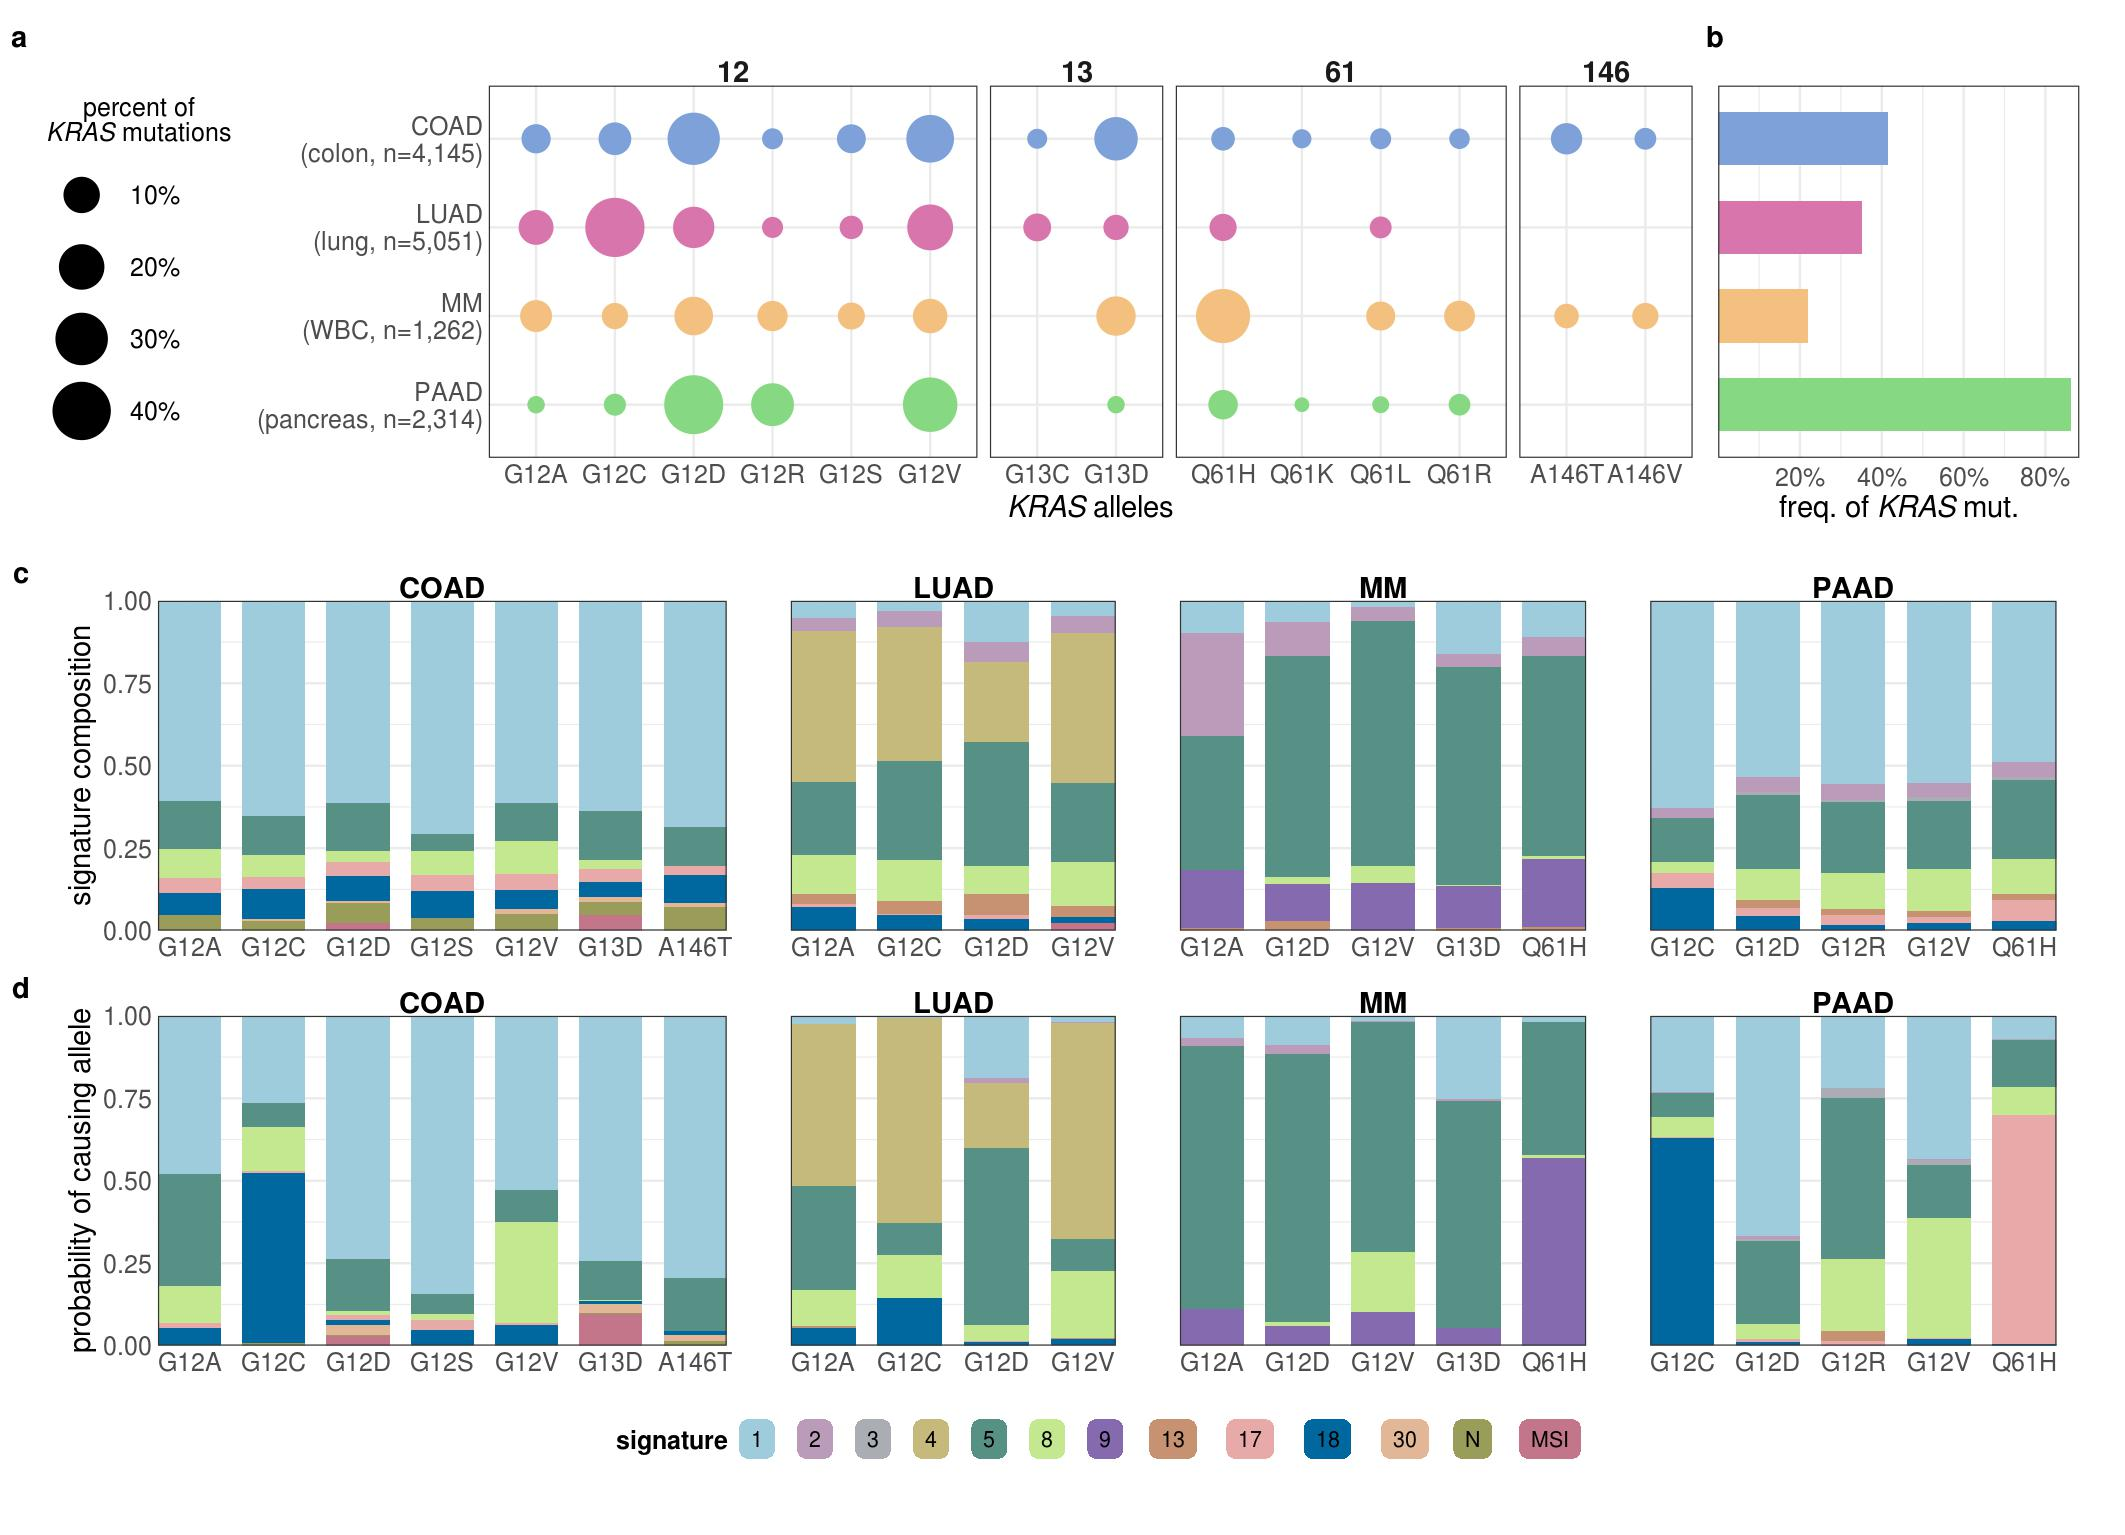
\includegraphics[width=180mm]{figures/Fig_1.jpeg}
\caption{
    \textbf{The contribution of mutational processes to \KRAS{} mutagenesis.}
    \textbf{a.} The distribution of \KRAS{} allele frequencies at the four hotspots, codons 12 (left), 13 (middle-left), 61 (middle-right), and 146 (right) in each cancer. The size of the circle reflects the percent of \KRAS{} mutations that are the indicated allele in each cancer. Each cancer is assigned a different color. The number of tumor samples whose sequencing data was collected for this study is indicated along the y-axis. 
    \textbf{b.} The frequency of \KRAS{} mutations in each cancer.
    \textbf{c.} The average levels of mutational signatures in tumor samples separated by \KRAS{} allele. Each color represents a different mutational signature.
    \textbf{d.} The average probability of each mutational signature to have caused the \KRAS{} mutation in a tumor sample. This value accounts for the level of each mutational signature in the tumor sample and the ability of the mutational signature to cause the indicated \KRAS{} allele.
    \textbf{e.} The predicted vs. observed frequency of \KRAS{} alleles for all common alleles of each cancer. $\blacktriangle$ indicates the rejection of the null hypothesis that the observed and predicted frequencies are the same (Chi-squared test, p < 0.05). $\bullet$ indicates the failure to reject the null hypothesis (Chi-squared test, p $\ge$ 0.05). Error bars indicate 95\% confidence intervals of the predicted values.
}
\label{fig:mutational-signatures-main}
\end{figure}
\newpage


\begin{figure}[h!]
\centering
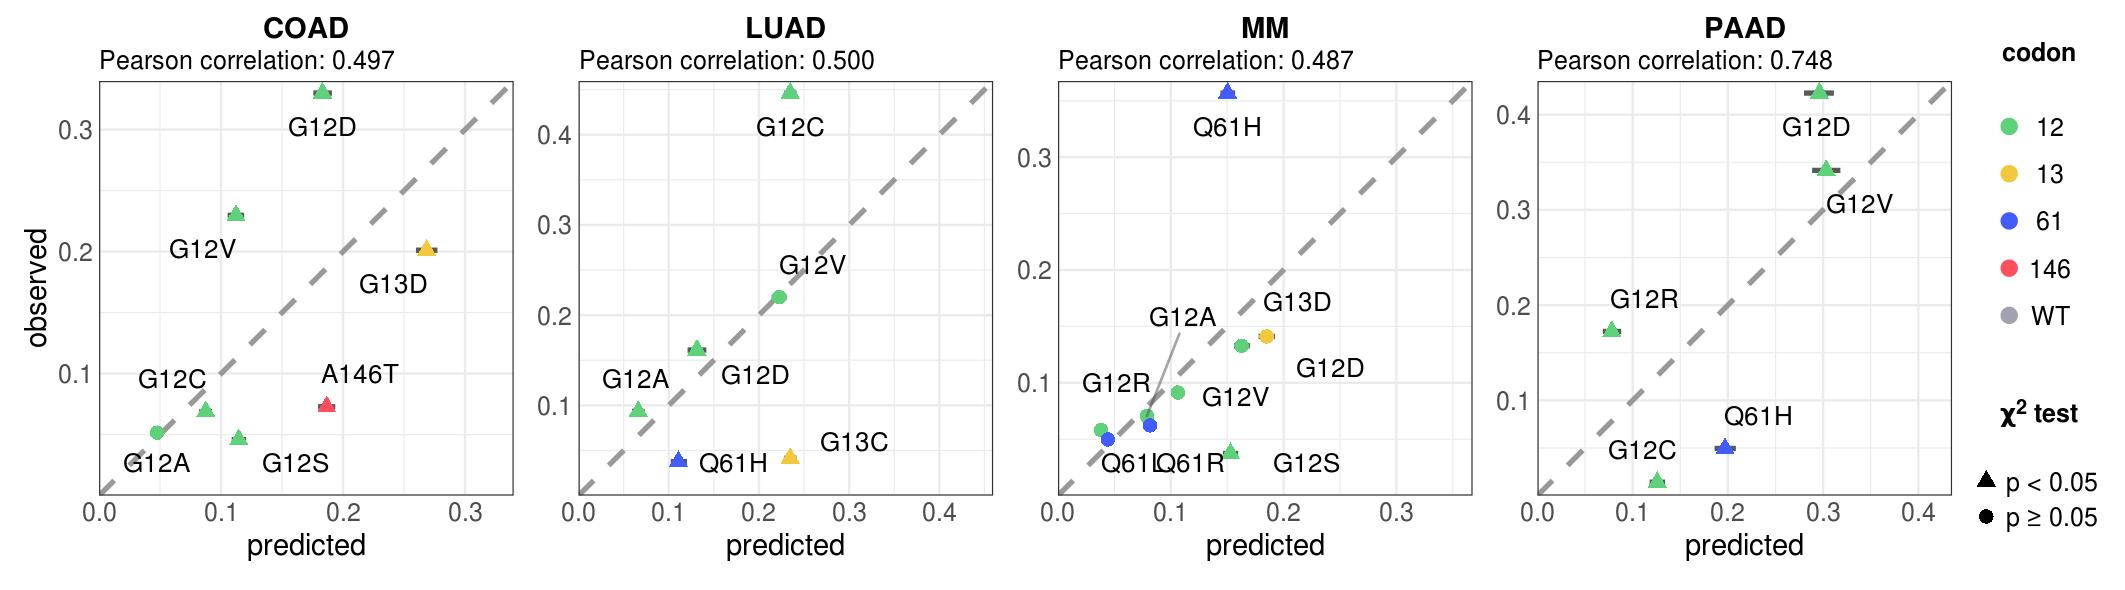
\includegraphics[width=180mm]{figures/Fig_2.jpeg}
\caption{The comutation networks of oncogenic \KRAS{} alleles.}
\label{fig:comutation-main}
\end{figure}

\newpage
\noindent \textbf{Figure 2. The comutation networks of oncogenic \KRAS{} alleles.}
\textbf{a.} The comutation network of the \KRAS{} alleles in COAD with each edge representing a comutation interaction between an allele and another gene. The color of the edge indicates whether the interaction was an increase (blue) or decrease (green) in the frequency of comutation.
\textbf{b.} A subset of the network shown in \textbf{a} of genes known to physically interact with \KRAS{}, are in one of its canonical up- or downstream pathways, or are validated oncogenes. The width of the edge indicates the strength of the association.
\textbf{c.} Cellular functions enriched in the comutation networks of the \KRAS{} alleles in COAD (left), LUAD (center), and PAAD (right). The size of the dot indicates the number of genes in both the function and the comutation network and the transparency indicates the p-value of the enrichment.
\textbf{d, e.} A visualization of the increased (\textbf{d}) or decreased (\textbf{e}) comutation of select genes with \KRAS{} G12D in COAD. Rows of the central plot represent genes. Each column of the central plot is a different tumor sample. A filled space denotes a mutation of the gene in the sample, the color describing the type of variant. The bar plots above and to the right indicate the marginal values of the central plot.
\textbf{f.} A comparison of the comutation rates of the genes producing proteins in the PPIN of SMAD1-3. Each column is a gene with a comutation interaction with a \KRAS{} allele and in at least one of the gene sets. The black tiles on top indicate that the gene was in the PPIN of the indicated SMAD protein. The bar plot shows the distribution of the comutation events of each gene across tumor samples with the various \KRAS{} mutations.
\newpage


\begin{figure}[h!]
\centering
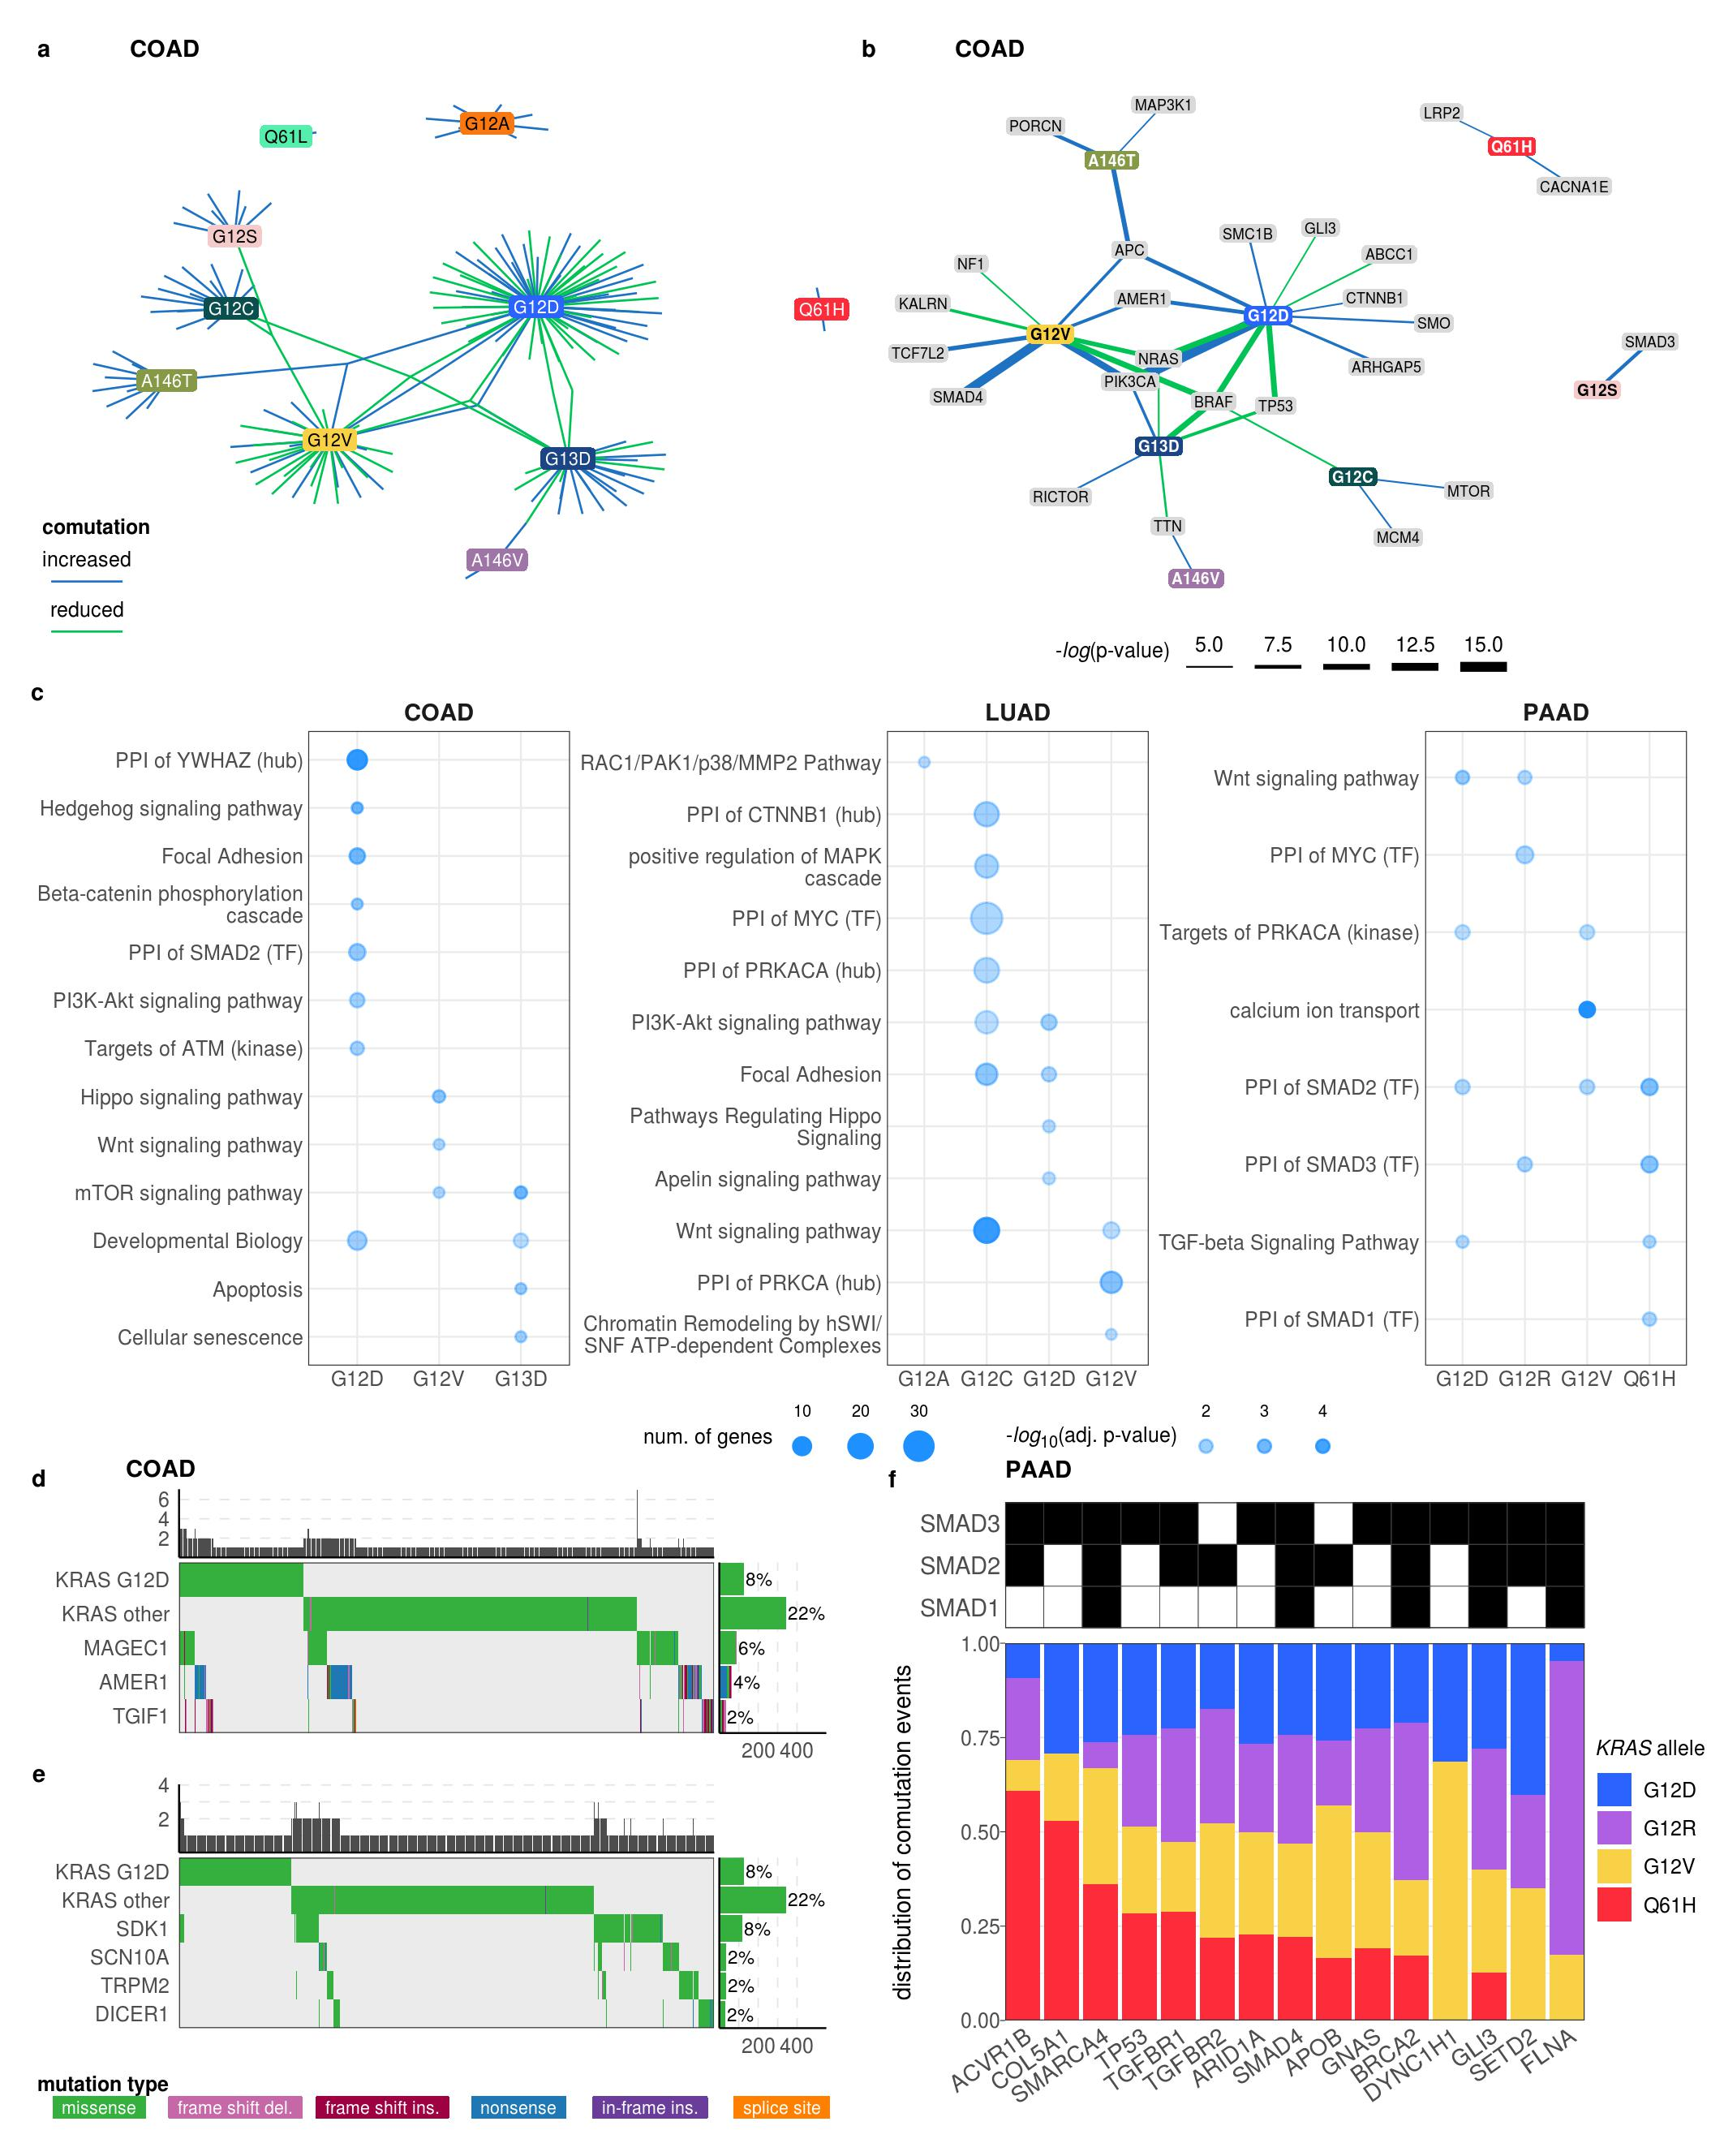
\includegraphics[width=180mm]{figures/Fig_3.jpeg}
\caption{
    \textbf{Allele-specific genetic dependencies in COAD cell lines.}
    \textbf{a.} Gene sets with significant enrichment for increased (lower dependency score; purple) or reduced (higher dependency score; orange) genetic dependency in COAD cell lines. The size of the dot relates the p-value of the association and the color indicated the strength of the enrichment ("normalized enrichment score").
    \textbf{b, c.} Heatmaps ranking the cell lines by dependency score of the genes at the leading edge of enrichment for two gene sets. Each row represents a gene and each cell represents a cell line colored by its \KRAS{} allele. The cell lines were arranged in ranking order by their dependency score for the gene. Thus, each column indicates a rank. The line plots above the heatmaps indicate the representation (density) of each \KRAS{} allele at each rank across the genes.
    \textbf{d.} Clustered heatmaps of the genes that demonstrated differential genetic dependency amongst cell lines of different \KRAS{} alleles in COAD cell lines. Each column is a cell line labeled by its DepMap ID and each row is a gene.
    \textbf{e.} Examples of genes that demonstrated differential genetic dependency amongst cell lines of different \KRAS{} alleles in COAD (*: p<0.05, **: p<0.01, ***: p<0.001; p-values were adjusted using the Benjamini-Hochberg FDR correction method).
}
\label{fig:coad-dependency-main}
\end{figure}
\newpage


\begin{figure}[h!]
\centering
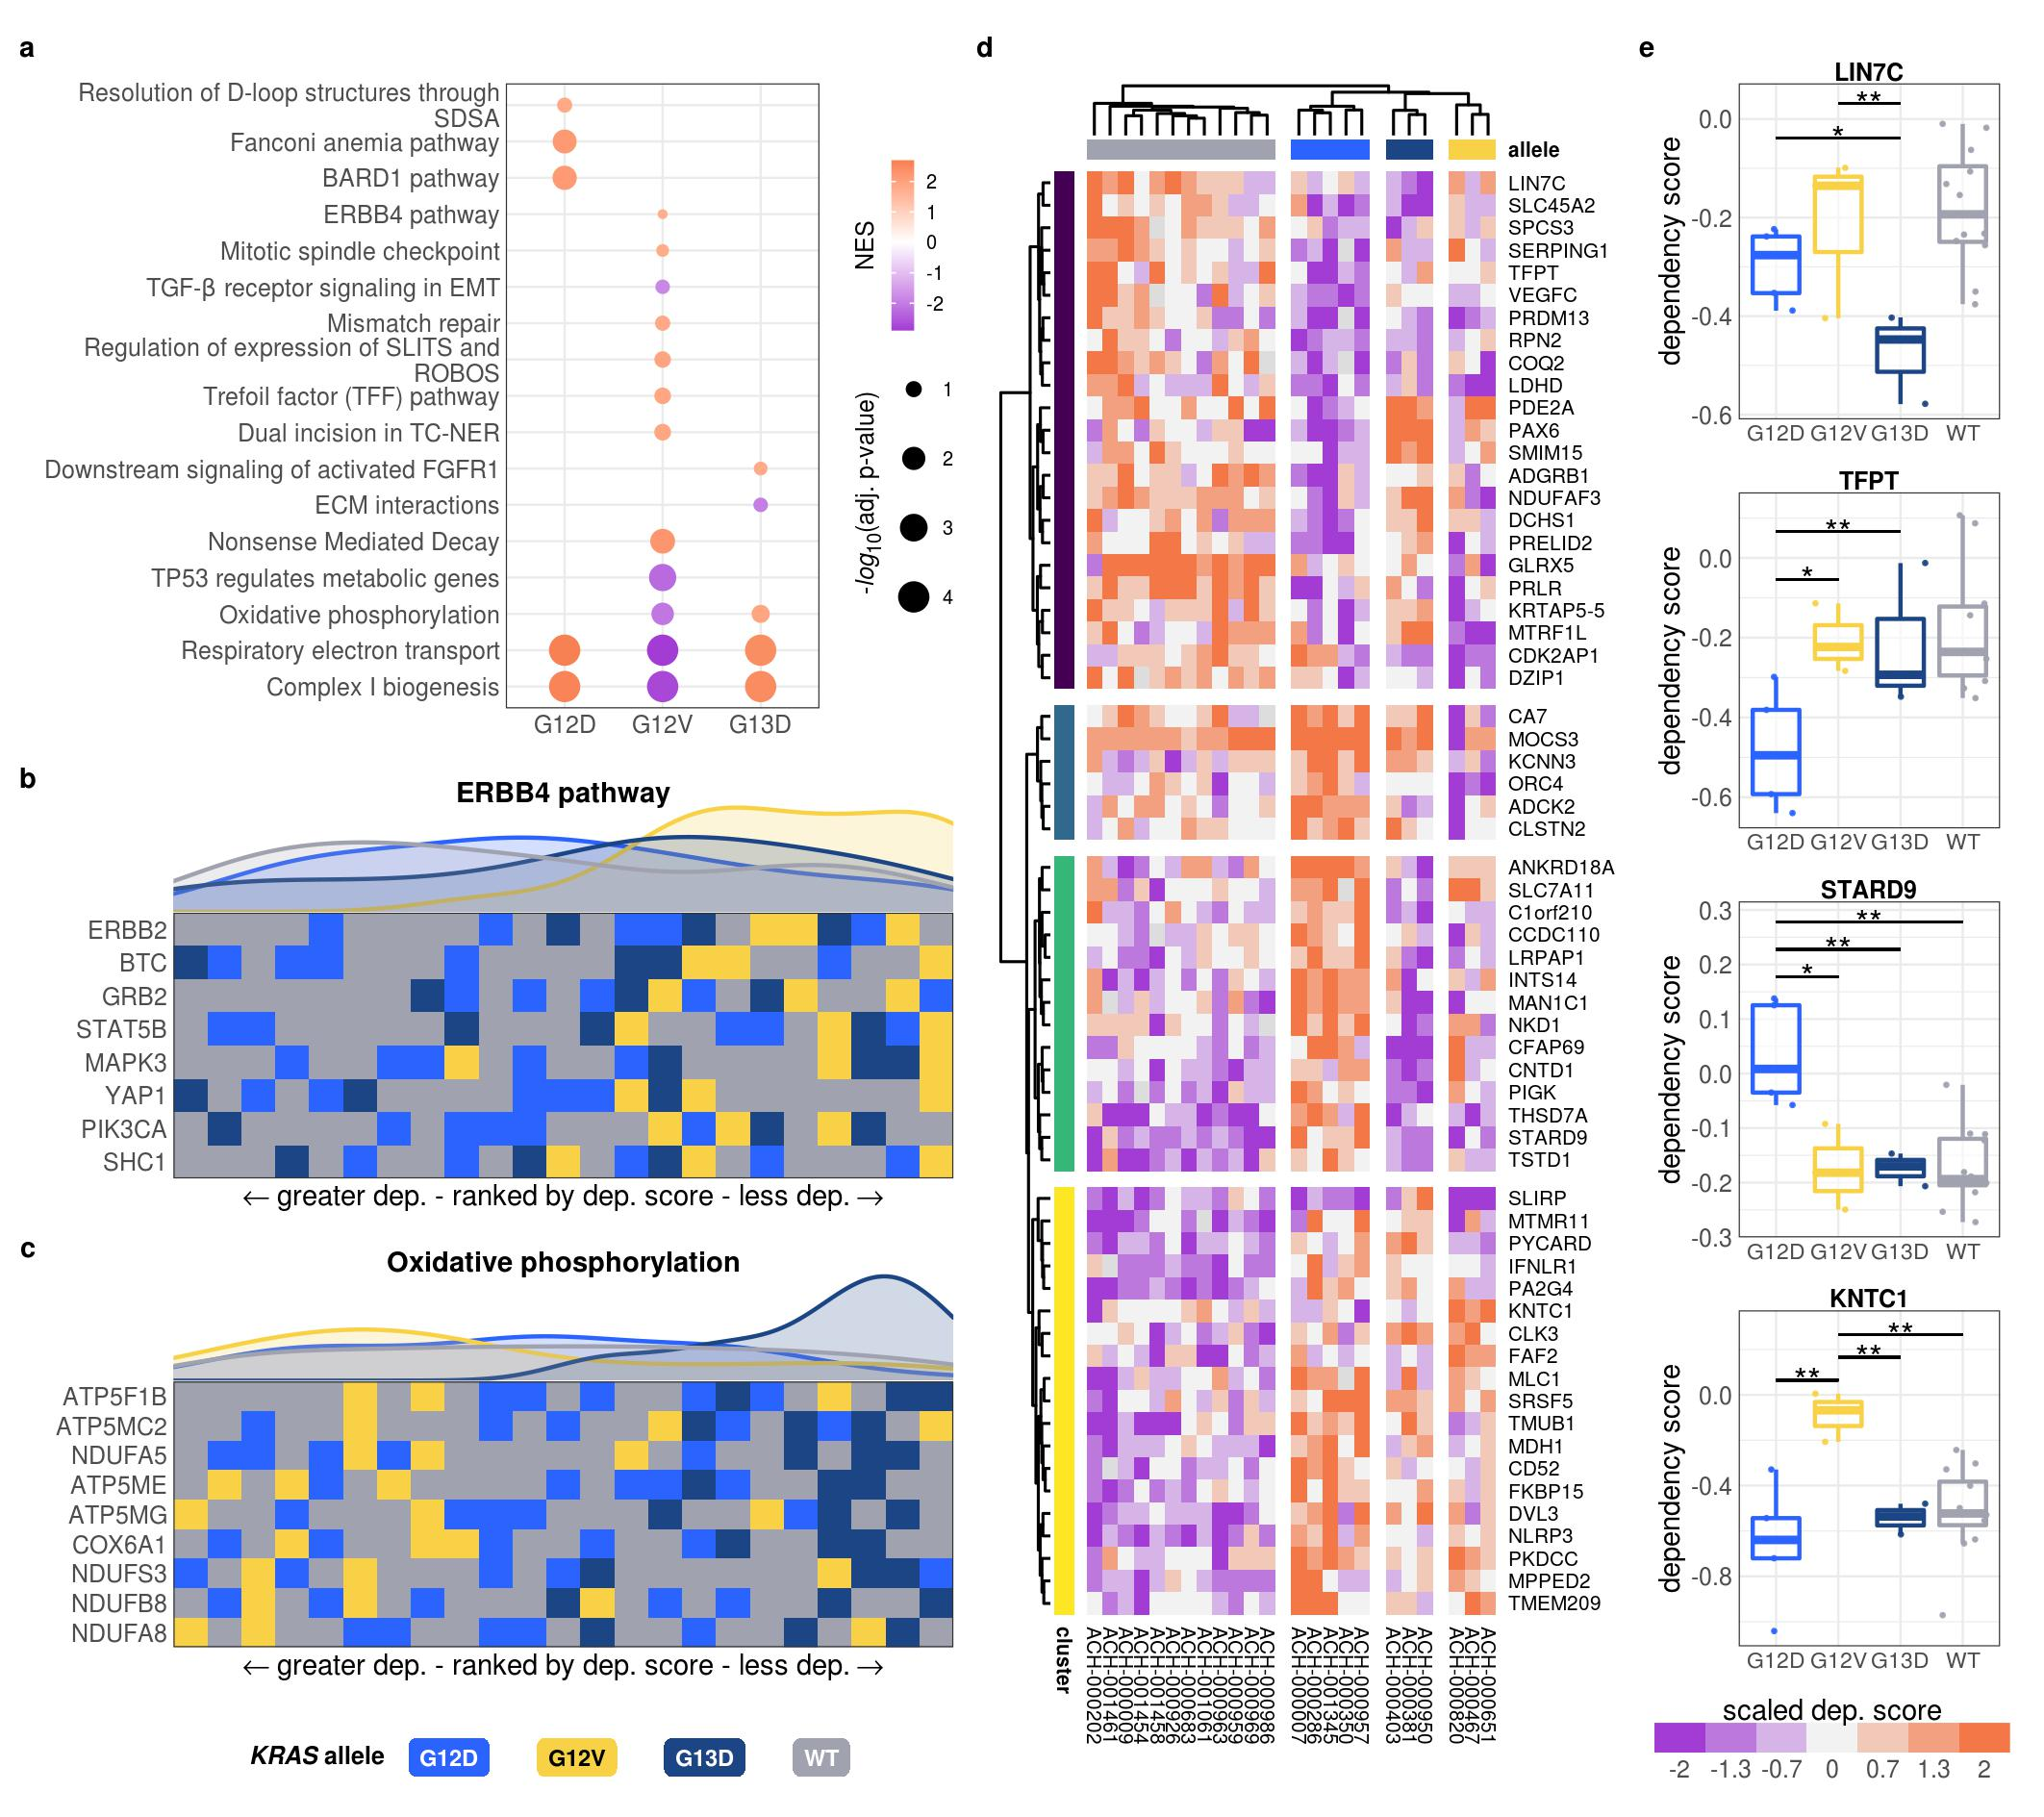
\includegraphics[width=180mm]{figures/Fig_4.jpeg}
\caption{Integration of comutation and genetic dependency results.}
\label{fig:results-integration-main}
\end{figure}

\newpage
\noindent \textbf{Figure 4. Integration of comutation and genetic dependency results.}
\textbf{a.} A table of the genes found to comutate and demonstrate differential dependency with the same \KRAS{} allele and cancer. The "Dependency comparison" indicates the comparison of dependency scores found to be statistically significant; the "Adj. p-value" is the Benjamini-Hochberg-adjusted p-value for the comparison. The "Comutation interaction" indicates if the comutation interaction was a reduced or increased rate of comutation; the "P-value" is the p-value for this interaction.
\textbf{b.} The connectivity of the proteins encoded by the genes found to comutate or demonstrate differential dependence with each \KRAS{} allele on the PPIN. The right-most column represents the null distribution of the connectivity of randomly selected pairs of nodes. The bars indicate the distribution of the geodesic distances (shortest path length) between nodes in the PPIN.
\textbf{c.}The largest connected subnetworks of the PPIN of genes found to comutate or demonstrate differential dependence with a \KRAS{} allele in COAD was extracted and merged. Nodes present in multiple subnetworks are colored shades of brown, save for prominent oncogenes and tumor suppressors in COAD, shown in red ("special"). The rest of the nodes are colored by which allele they are associated with. The edges share the color of the nodes they connect if the nodes are the same color, otherwise they are grey. Curated groups of proteins with related cellular functions are highlighted and labeled.
\newpage


\beginsupplement

\makeatletter
\renewcommand{\fnum@figure}{Supplementary \figurename~\thefigure}
\makeatother


\begin{figure}[h!]
\centering
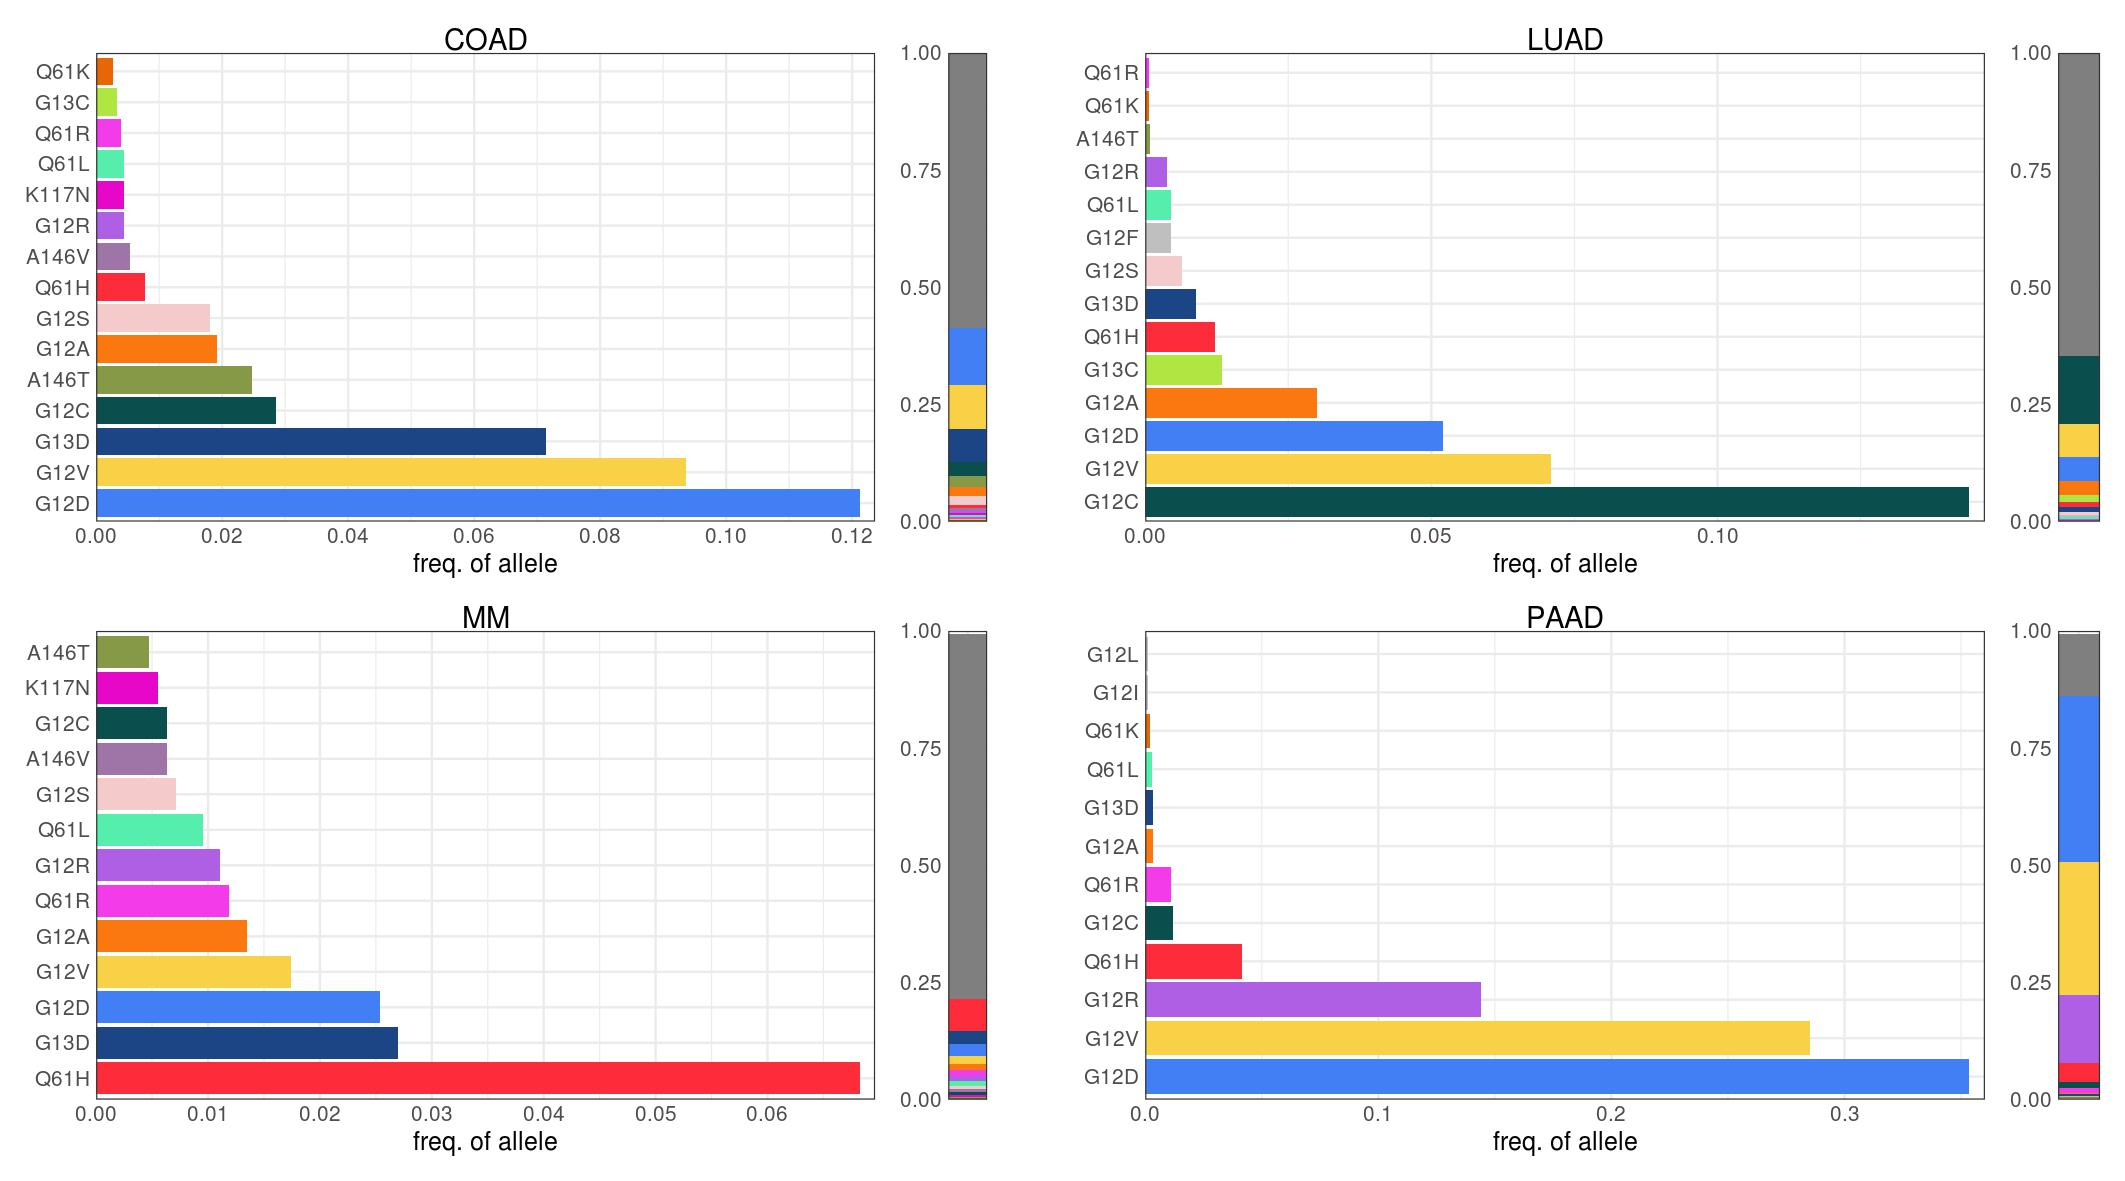
\includegraphics[width=180mm]{figures/Supp_Fig_1.jpeg}
\caption{
    \textbf{Mutational signatures in tumor samples.}
    \textbf{a, b.} The detected level of the mutational signatures in each tumor sample. In \textbf{a}, each tumor sample is a column.
    \textbf{c.} The average levels of clock (signatures 1 and 5) and non-clock (all other signatures) in the tumor samples.
}
\label{sfig:mutational-signatures-supp}
\end{figure}
\newpage


\begin{figure}[h!]
\centering
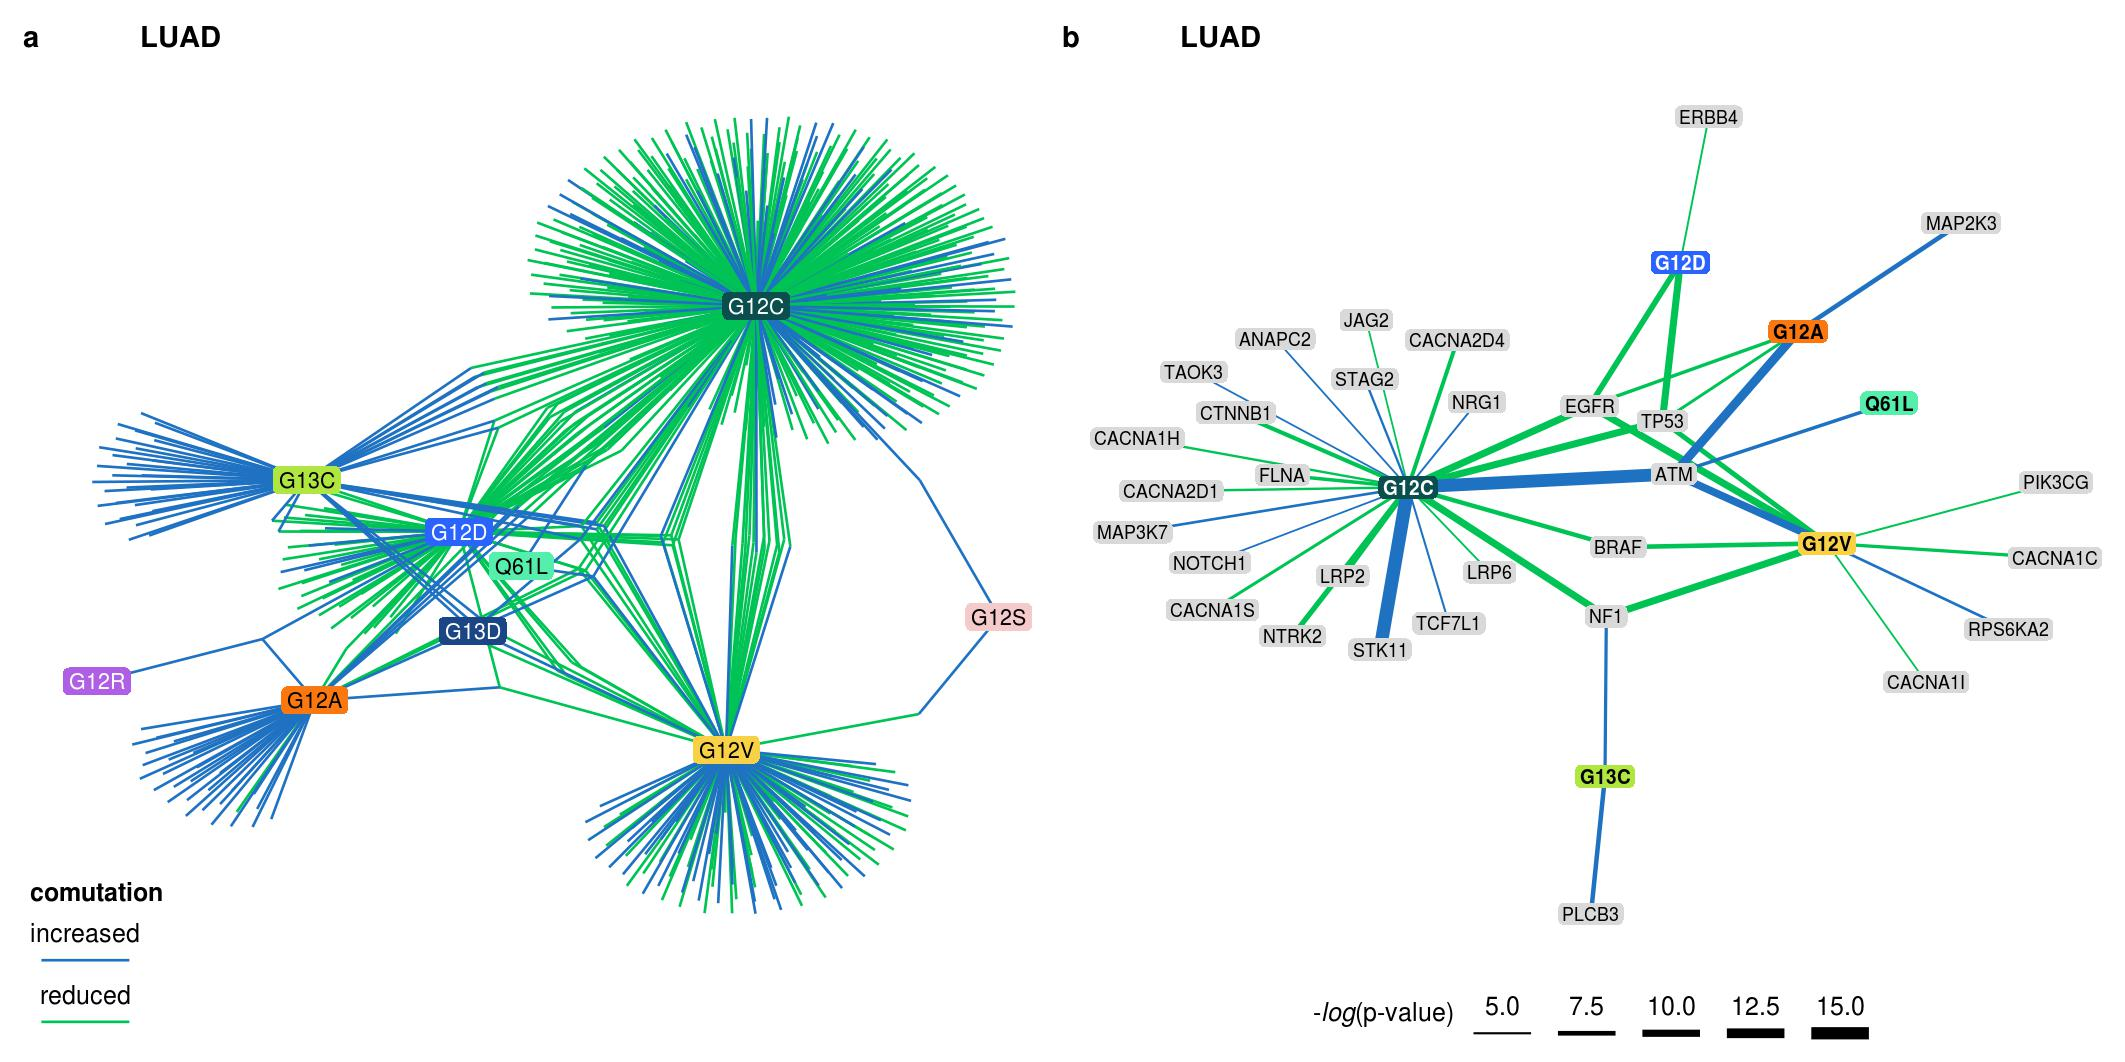
\includegraphics[width=180mm]{figures/Supp_Fig_2.jpeg}
\caption{
    \textbf{The comutation networks of \KRAS{} alleles in LUAD.}
    \textbf{a.} The comutation network of the \KRAS{} alleles in LUAD where each edge represents a comutation interaction between an allele and another gene. The color of the edge indicates whether the interaction was an increase (blue) or decrease (green) in the frequency of comutation.
    \textbf{b.} A subset of the network shown in \textbf{a} of genes in one of its canonical up- or downstream signaling pathways. The width of the edge indicates the strength of the association.
}
\label{sfig:luad-comutation-network}
\end{figure}
\newpage


\begin{figure}[h!]
\centering
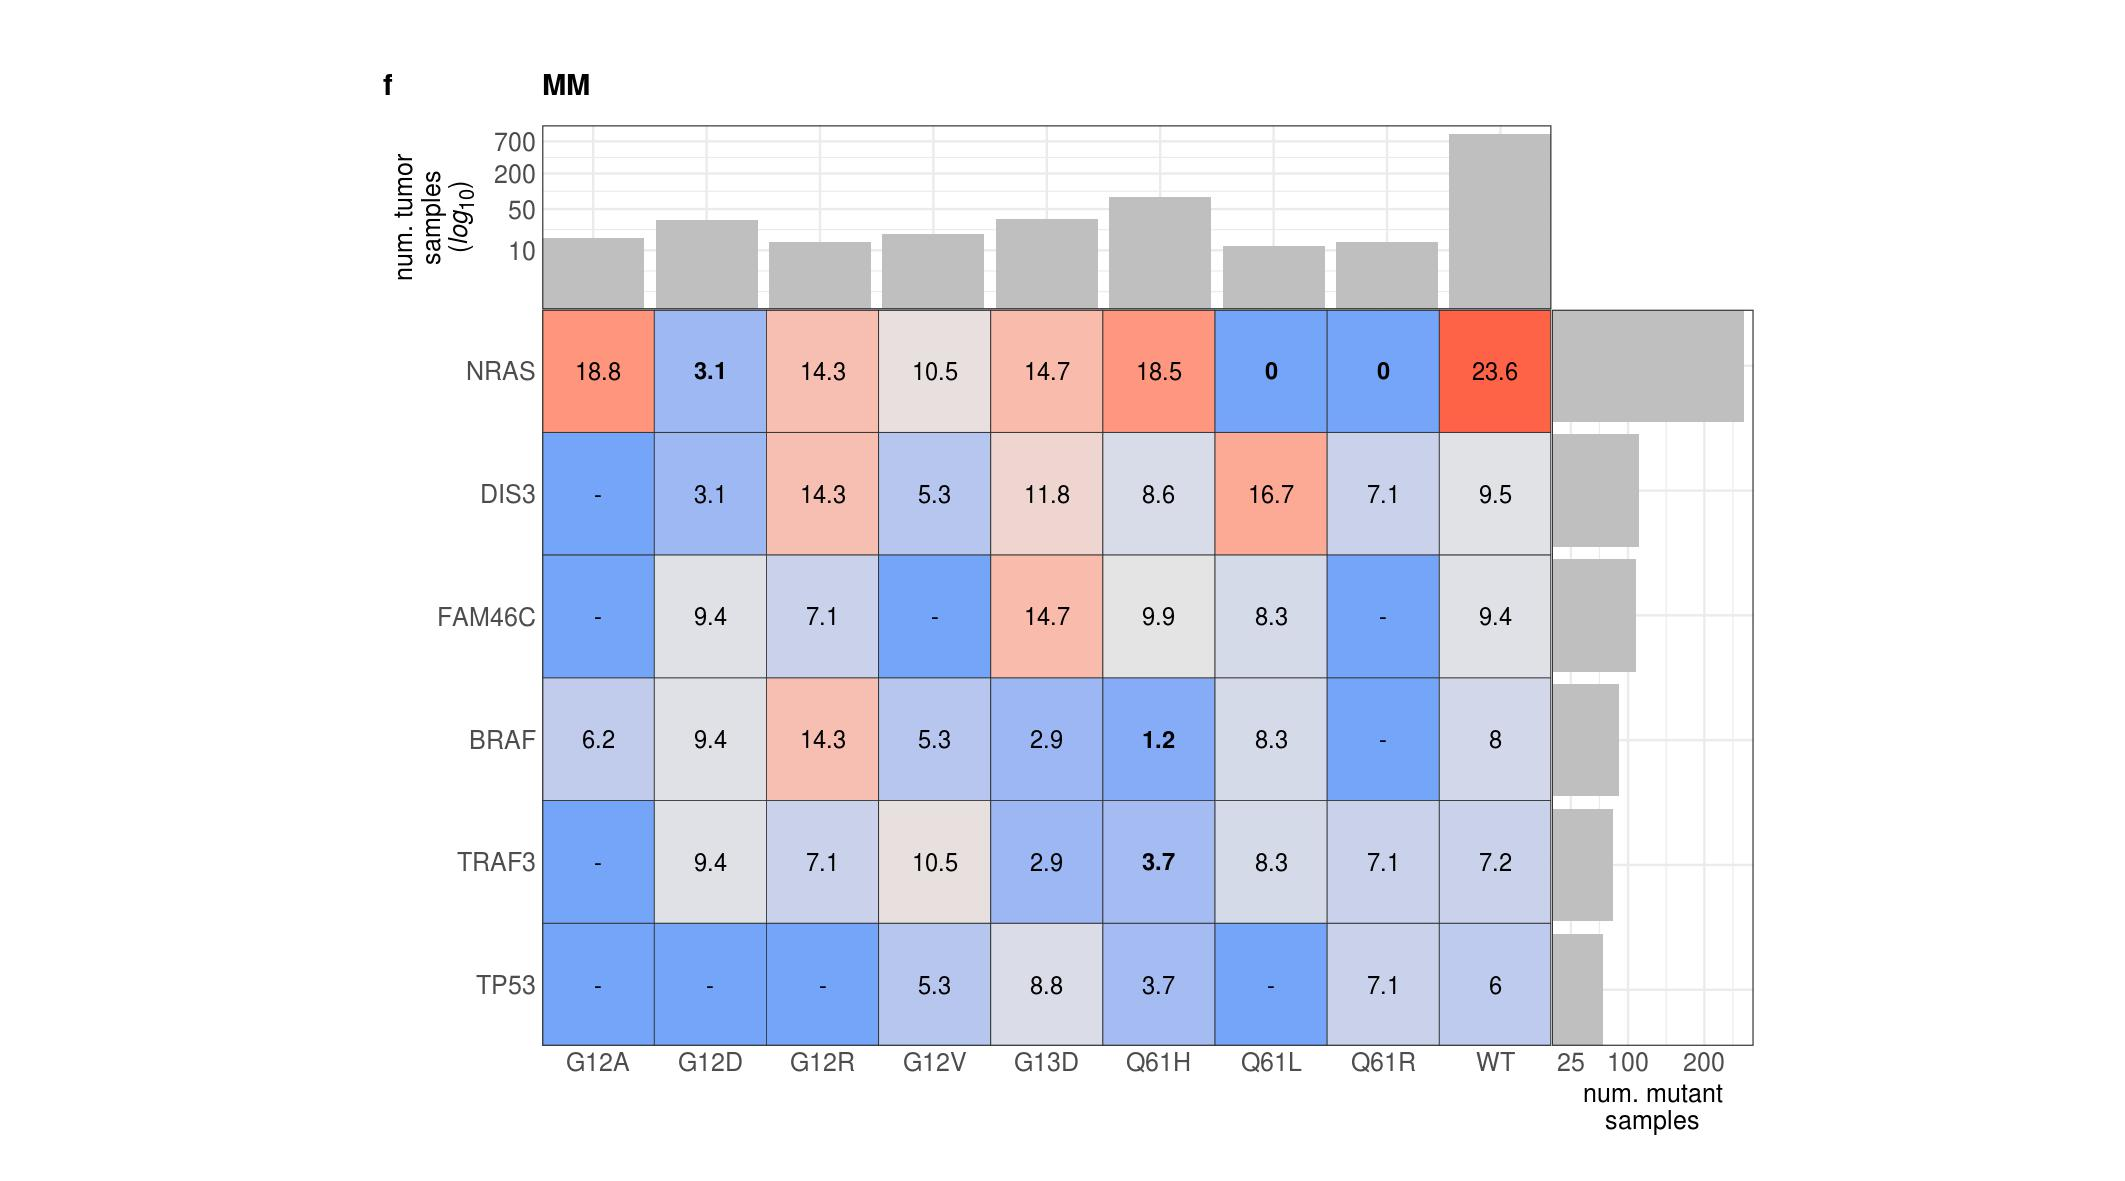
\includegraphics[width=180mm]{figures/Supp_Fig_3.jpeg}
\caption{
    \textbf{The comutation frequencies between known MM driving genes and \KRAS{} alleles.} The color is correlated with the comutation frequency (the fraction of cells with the \KRAS{} allele that also have a mutation in the other driver gene), indicated in each cell. Bold percent values indicate statistical significance of a comutation interaction (see Methods). The bar plot along the top indicates the number of samples with the \KRAS{} allele, and the bar plot on the right indicates the number of samples with a mutation in the gene.
}
\label{sfig:mm-comutation-heatmap}
\end{figure}
\newpage


\begin{figure}[h!]
\centering
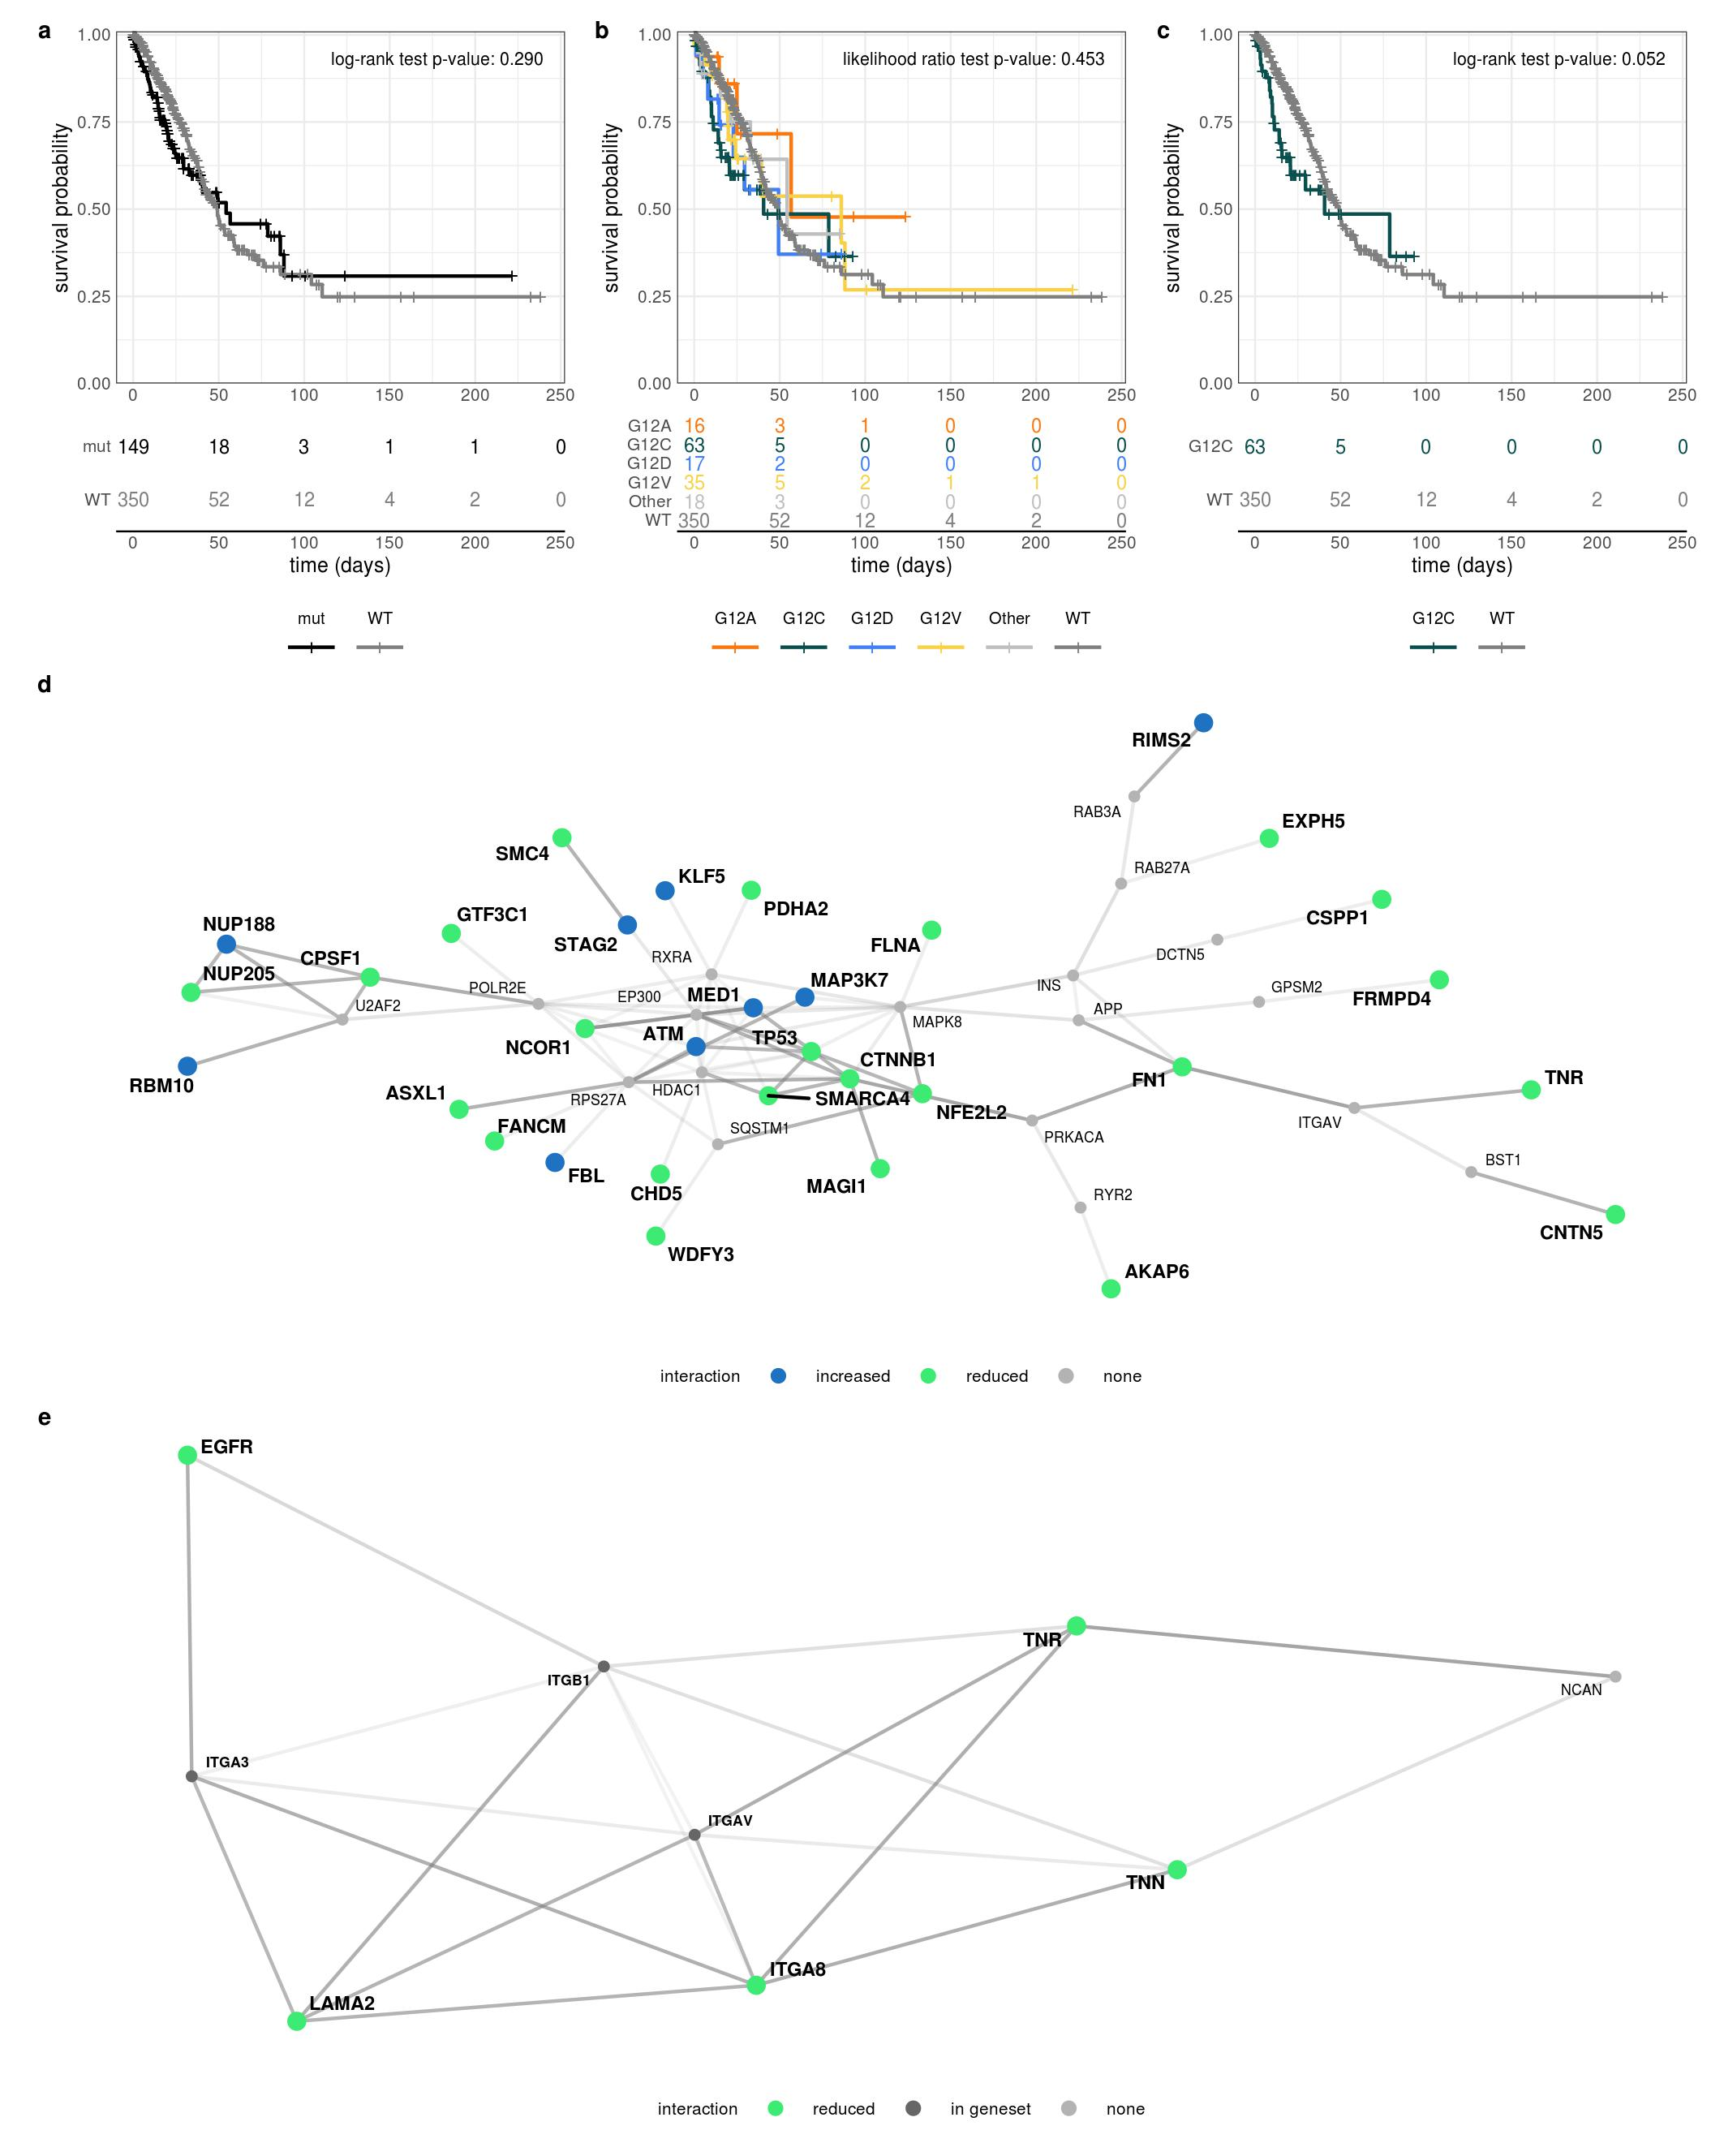
\includegraphics[width=180mm]{figures/Supp_Fig_4.jpeg}
\caption{
    \textbf{The comutation networks of \KRAS{} alleles in PAAD.}
    \textbf{a.} The comutation network of the \KRAS{} alleles in PAAD where each edge represents a comutation interaction between an allele and another gene. The color of the edge indicates whether the interaction was an increase (blue) or decrease (green) in the frequency of comutation.
    \textbf{b.} A subset of the network shown in \textbf{a} of genes known to physically interact with \KRAS{}, are in one of its canonical up- or downstream pathways, or are validated oncogenes. The width of the edge indicates the strength of the association.
    \textbf{c.} The log-odds of comutation between \KRAS{} alleles and other genes that had detectable opposing comutation interactions with multiple alleles.
}
\label{sfig:paad-comutation-network}
\end{figure}
\newpage


\begin{figure}[h!]
\centering
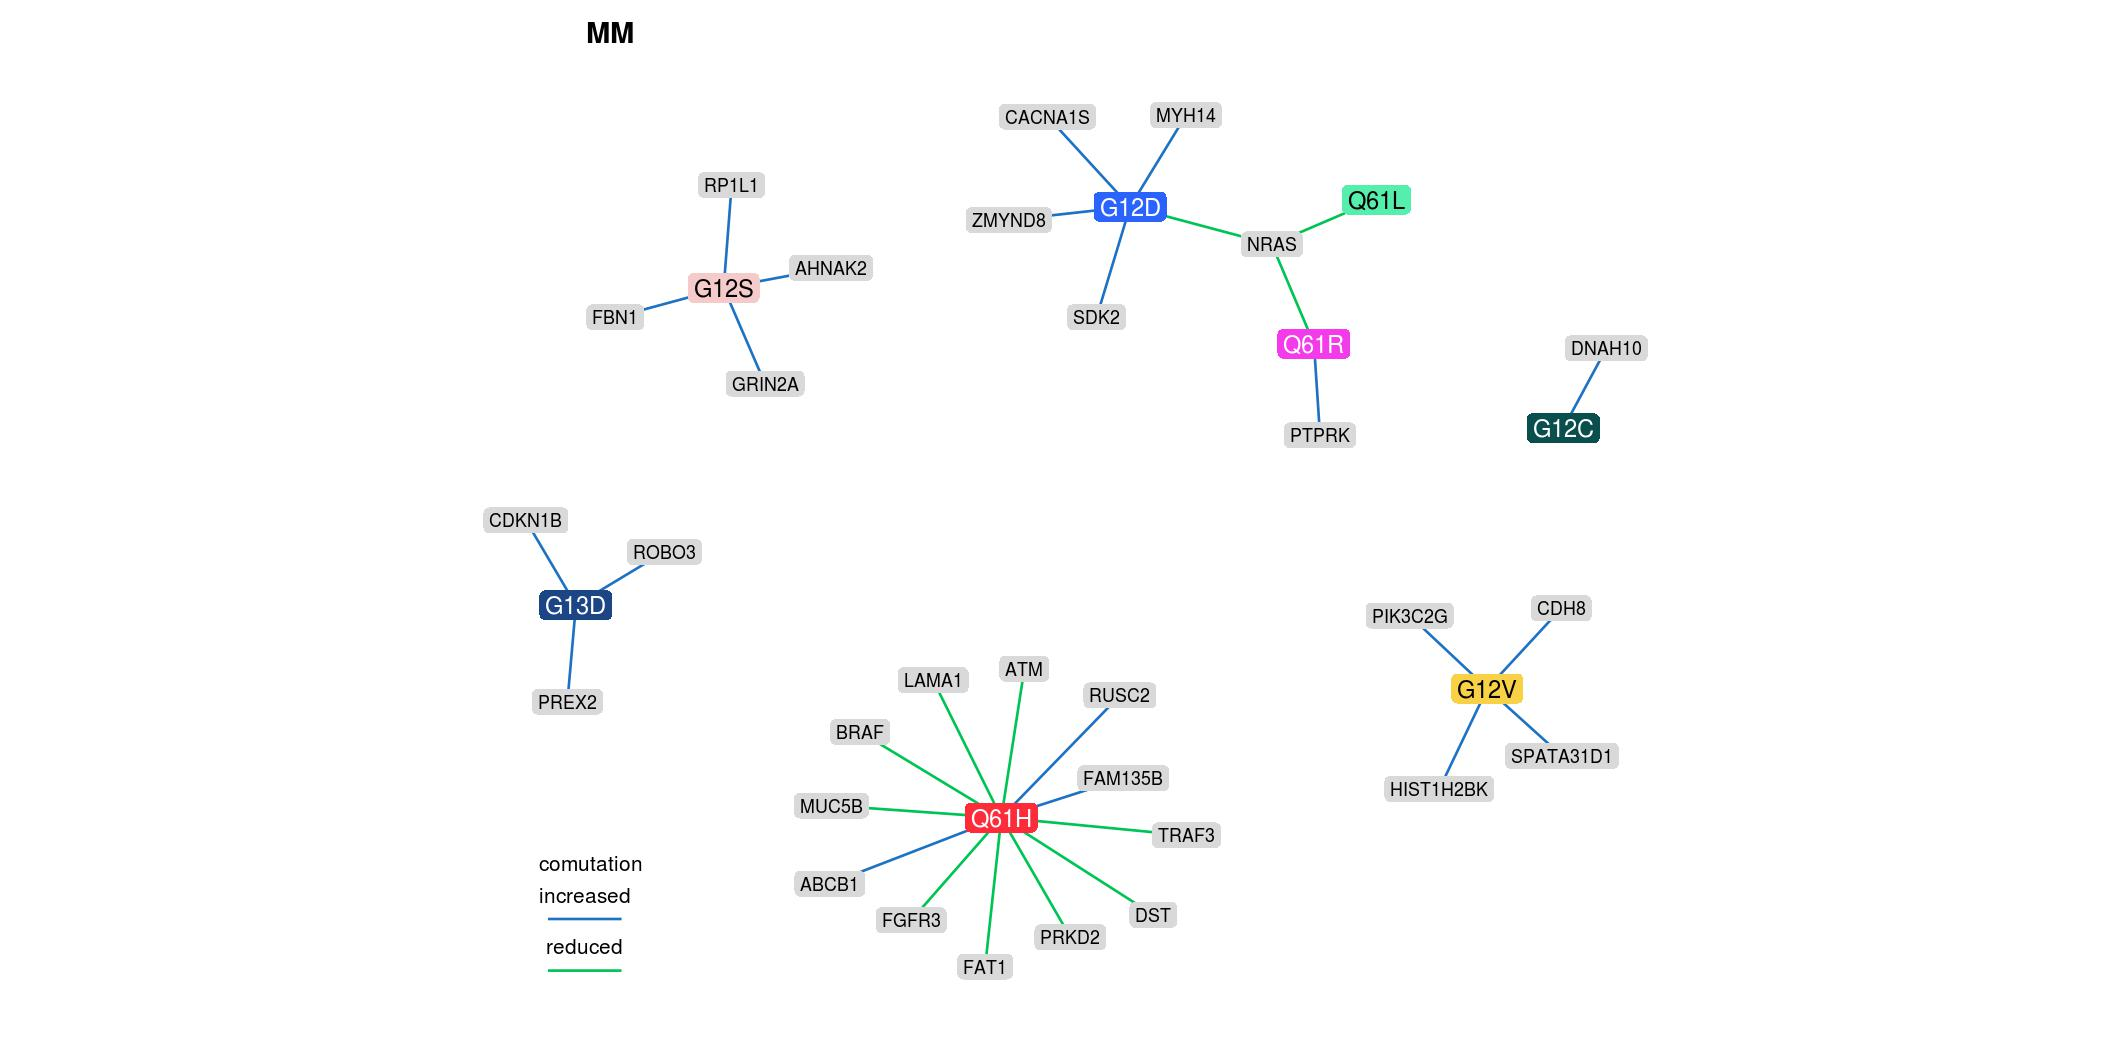
\includegraphics[width=180mm]{figures/Supp_Fig_5.jpeg}
\caption{
    \textbf{Gene sets with enriched genetic dependency in LUAD cell lines}
    \textbf{a, b.} Heatmaps ranking the cell lines by dependency score of the genes at the leading edge of enrichment for two gene sets in LUAD cell lines. Each row represents a gene and each cell represents a cell line colored by its \KRAS{} allele. The cell lines were arranged in ranking order by their dependency score for the gene. Thus, each column indicates a rank. The line plots above the heatmaps indicate the representation (density) of each \KRAS{} allele at each rank across the genes.
}
\label{sfig:luad-dependency-gsea}
\end{figure}
\newpage


\begin{figure}[h!]
\centering
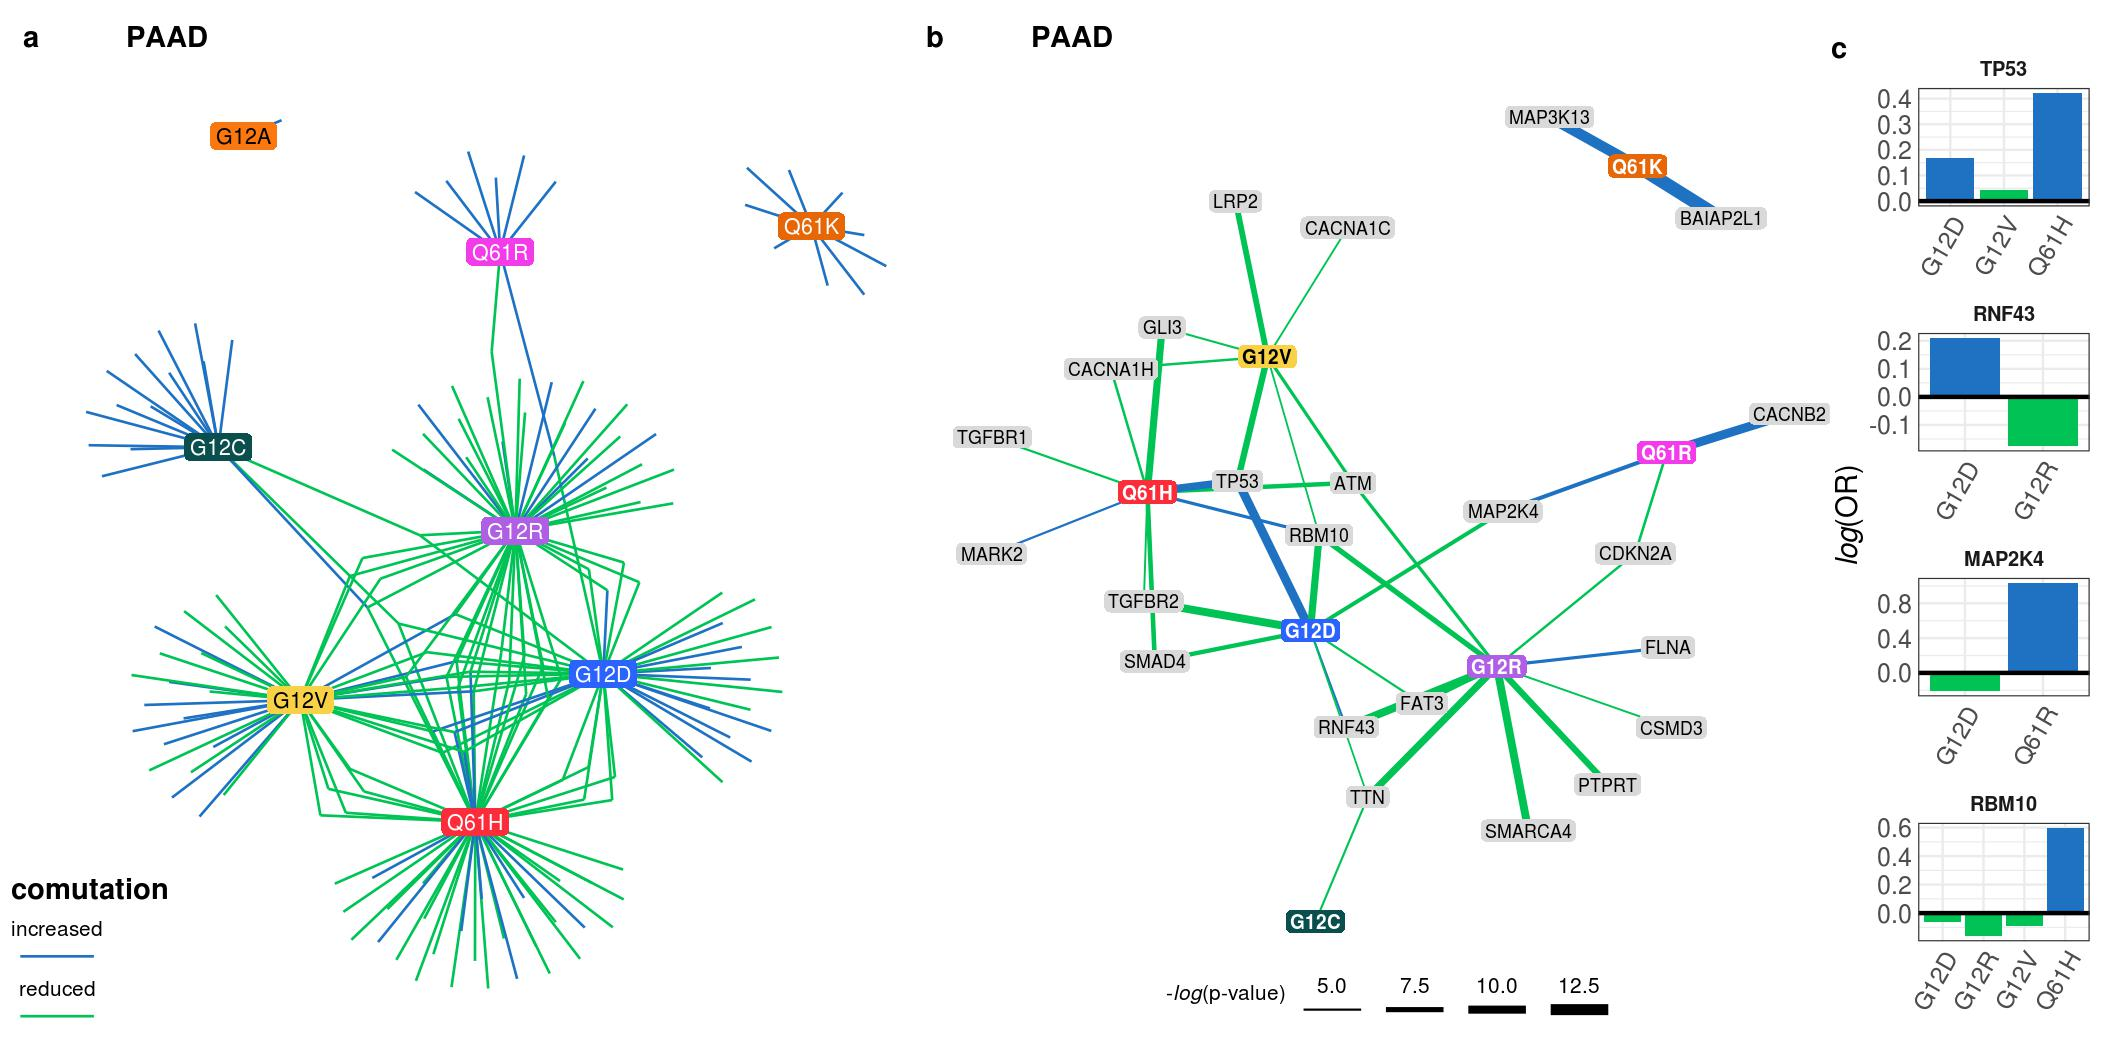
\includegraphics[width=88mm]{figures/Supp_Fig_6.jpeg}
\caption{Allele-specific genetic dependencies in LUAD cell lines.}
\label{sfig:luad-dependency-heatmap}
\end{figure}

\newpage
\noindent \textbf{Supplementary Figure 6. Allele-specific genetic dependencies in LUAD cell lines.}
Clustered heatmap of the genes that demonstrated differential genetic dependency amongst LUAD cell lines of different \KRAS{} alleles. Each column is a cell line labeled by its DepMap ID and each row is a gene. Only genes known to be involved in \KRAS{} signaling or previously implicated in driving cancer are labeled. Also, for visualization purposes, the scores of the WT cell lines were averaged into a single, representative group, labeled "WT (avg.)."
\newpage


\begin{figure}[h!]
\centering
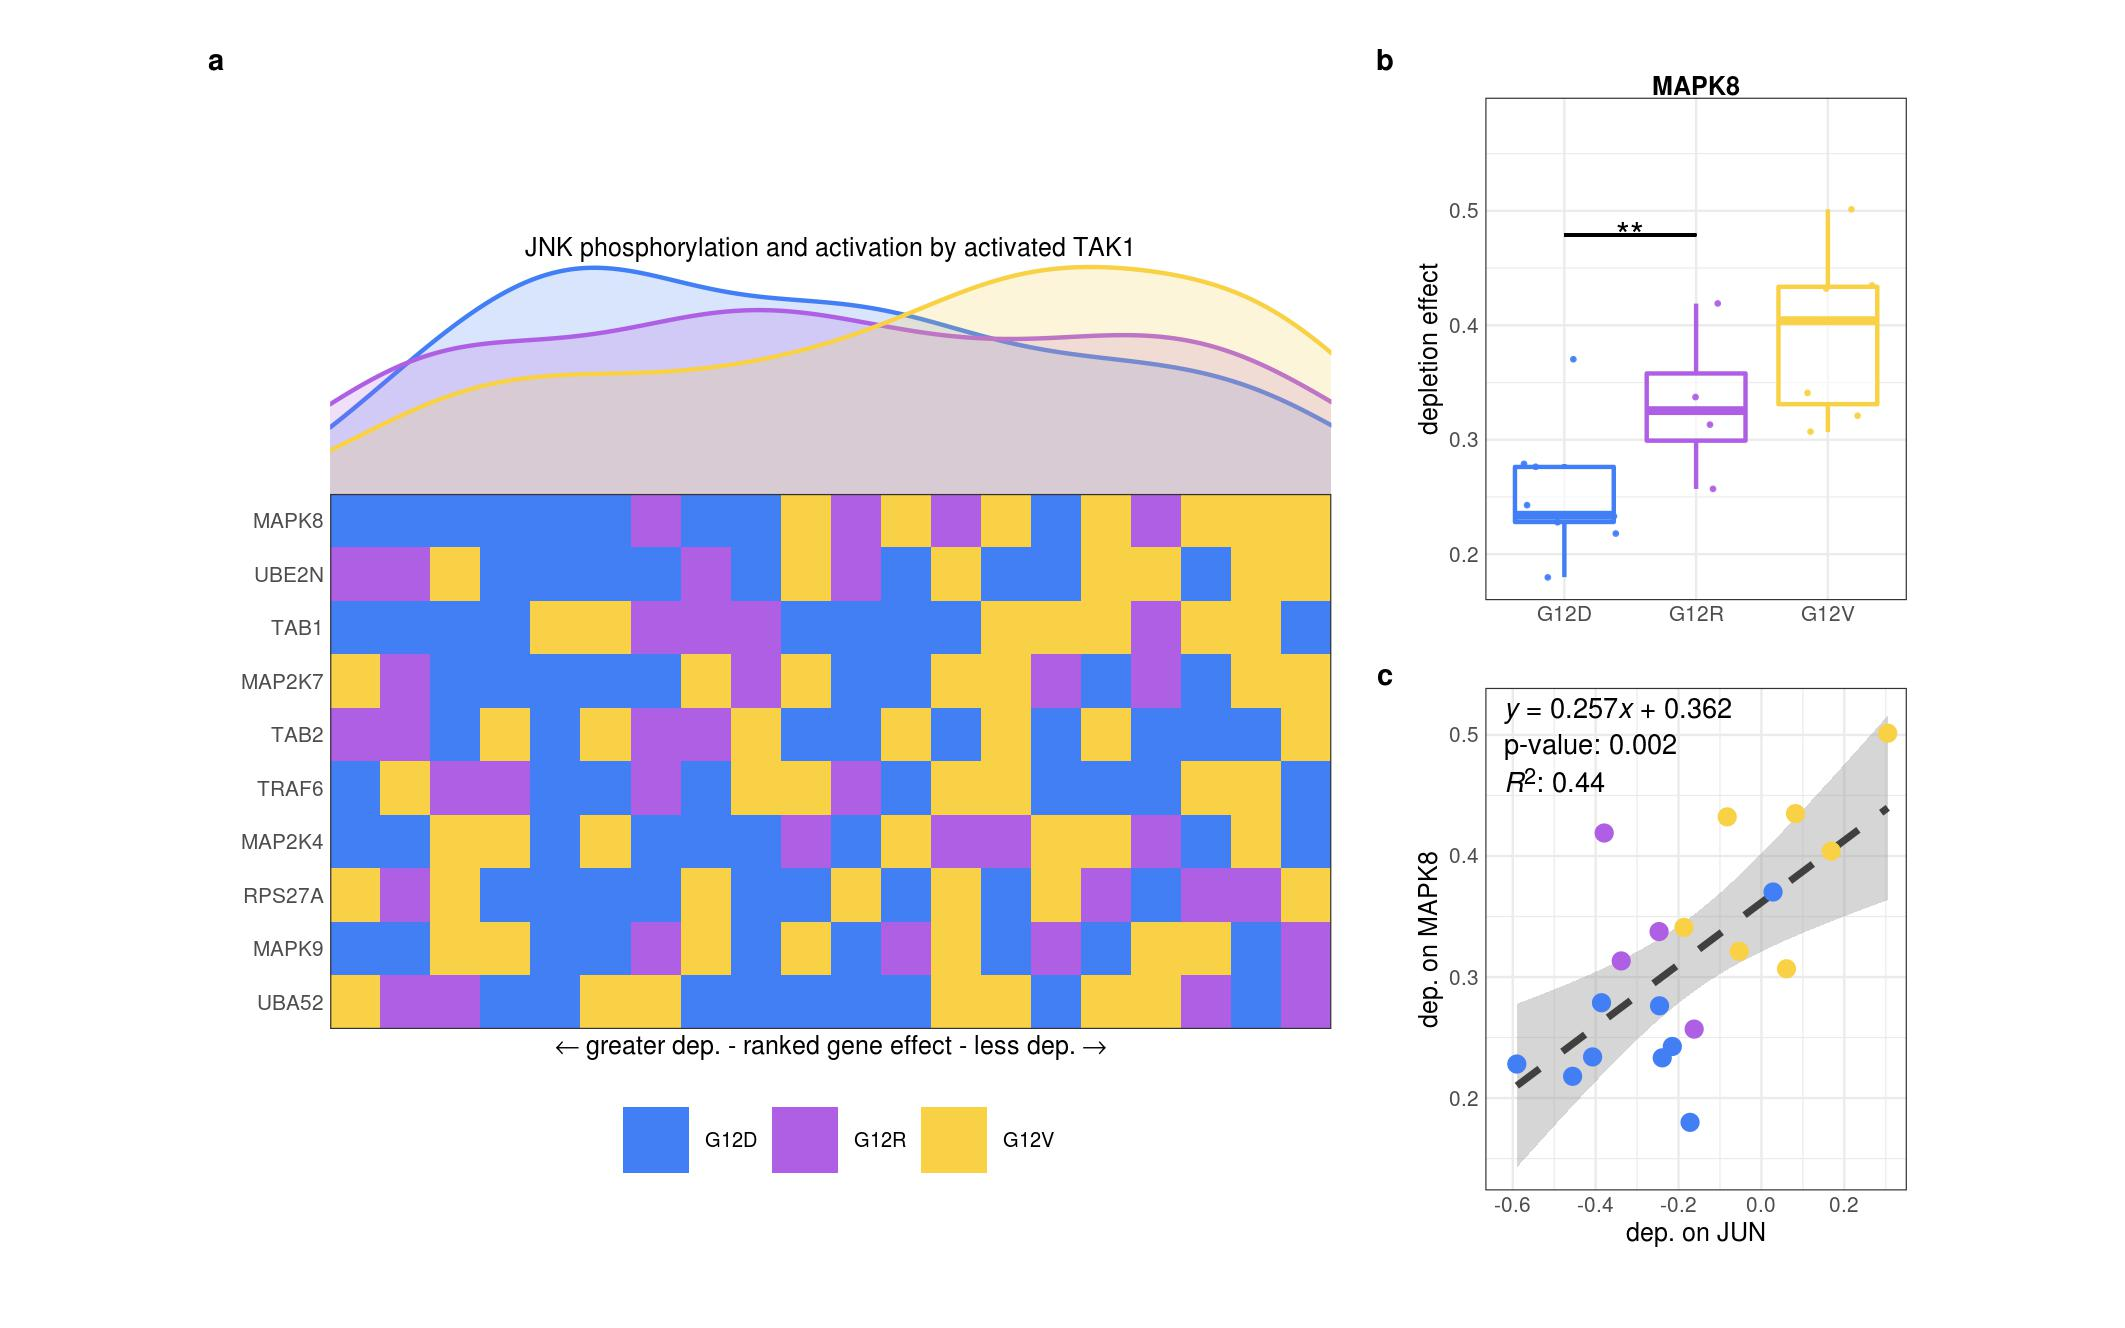
\includegraphics[width=88mm]{figures/Supp_Fig_7.jpeg}
\caption{Cellular processes enriched for greater or lesser genetic dependencies in PAAD cell lines separated by \KRAS{} allele.}
\label{sfig:paad-dependency-gsea}
\end{figure}

\newpage
\noindent \textbf{Supplementary Figure 7. Cellular processes enriched for greater or lesser genetic dependencies in PAAD cell lines separated by \KRAS{} allele.}
\textbf{a.} Gene sets with significant enrichment for increased (lower dependency score; purple) or reduced (higher dependency score; orange) genetic dependency in PAAD cell lines. The size of the dot relates the p-value of the association and the color indicated the strength of the enrichment.
\textbf{b, c, d.} Heatmaps ranking the cell lines by dependency score of genes at the leading edge of enrichment for three gene sets in PAAD. Each row represents a gene and each cell represents a cell line colored by its \KRAS{} allele. The cell lines were arranged in ranking order by their dependency score for the gene. Thus, each column indicates a rank. The line plots above the heatmaps indicate the representation (density) of each \KRAS{} allele at each rank across the genes.
\newpage


\begin{figure}[h!]
\centering
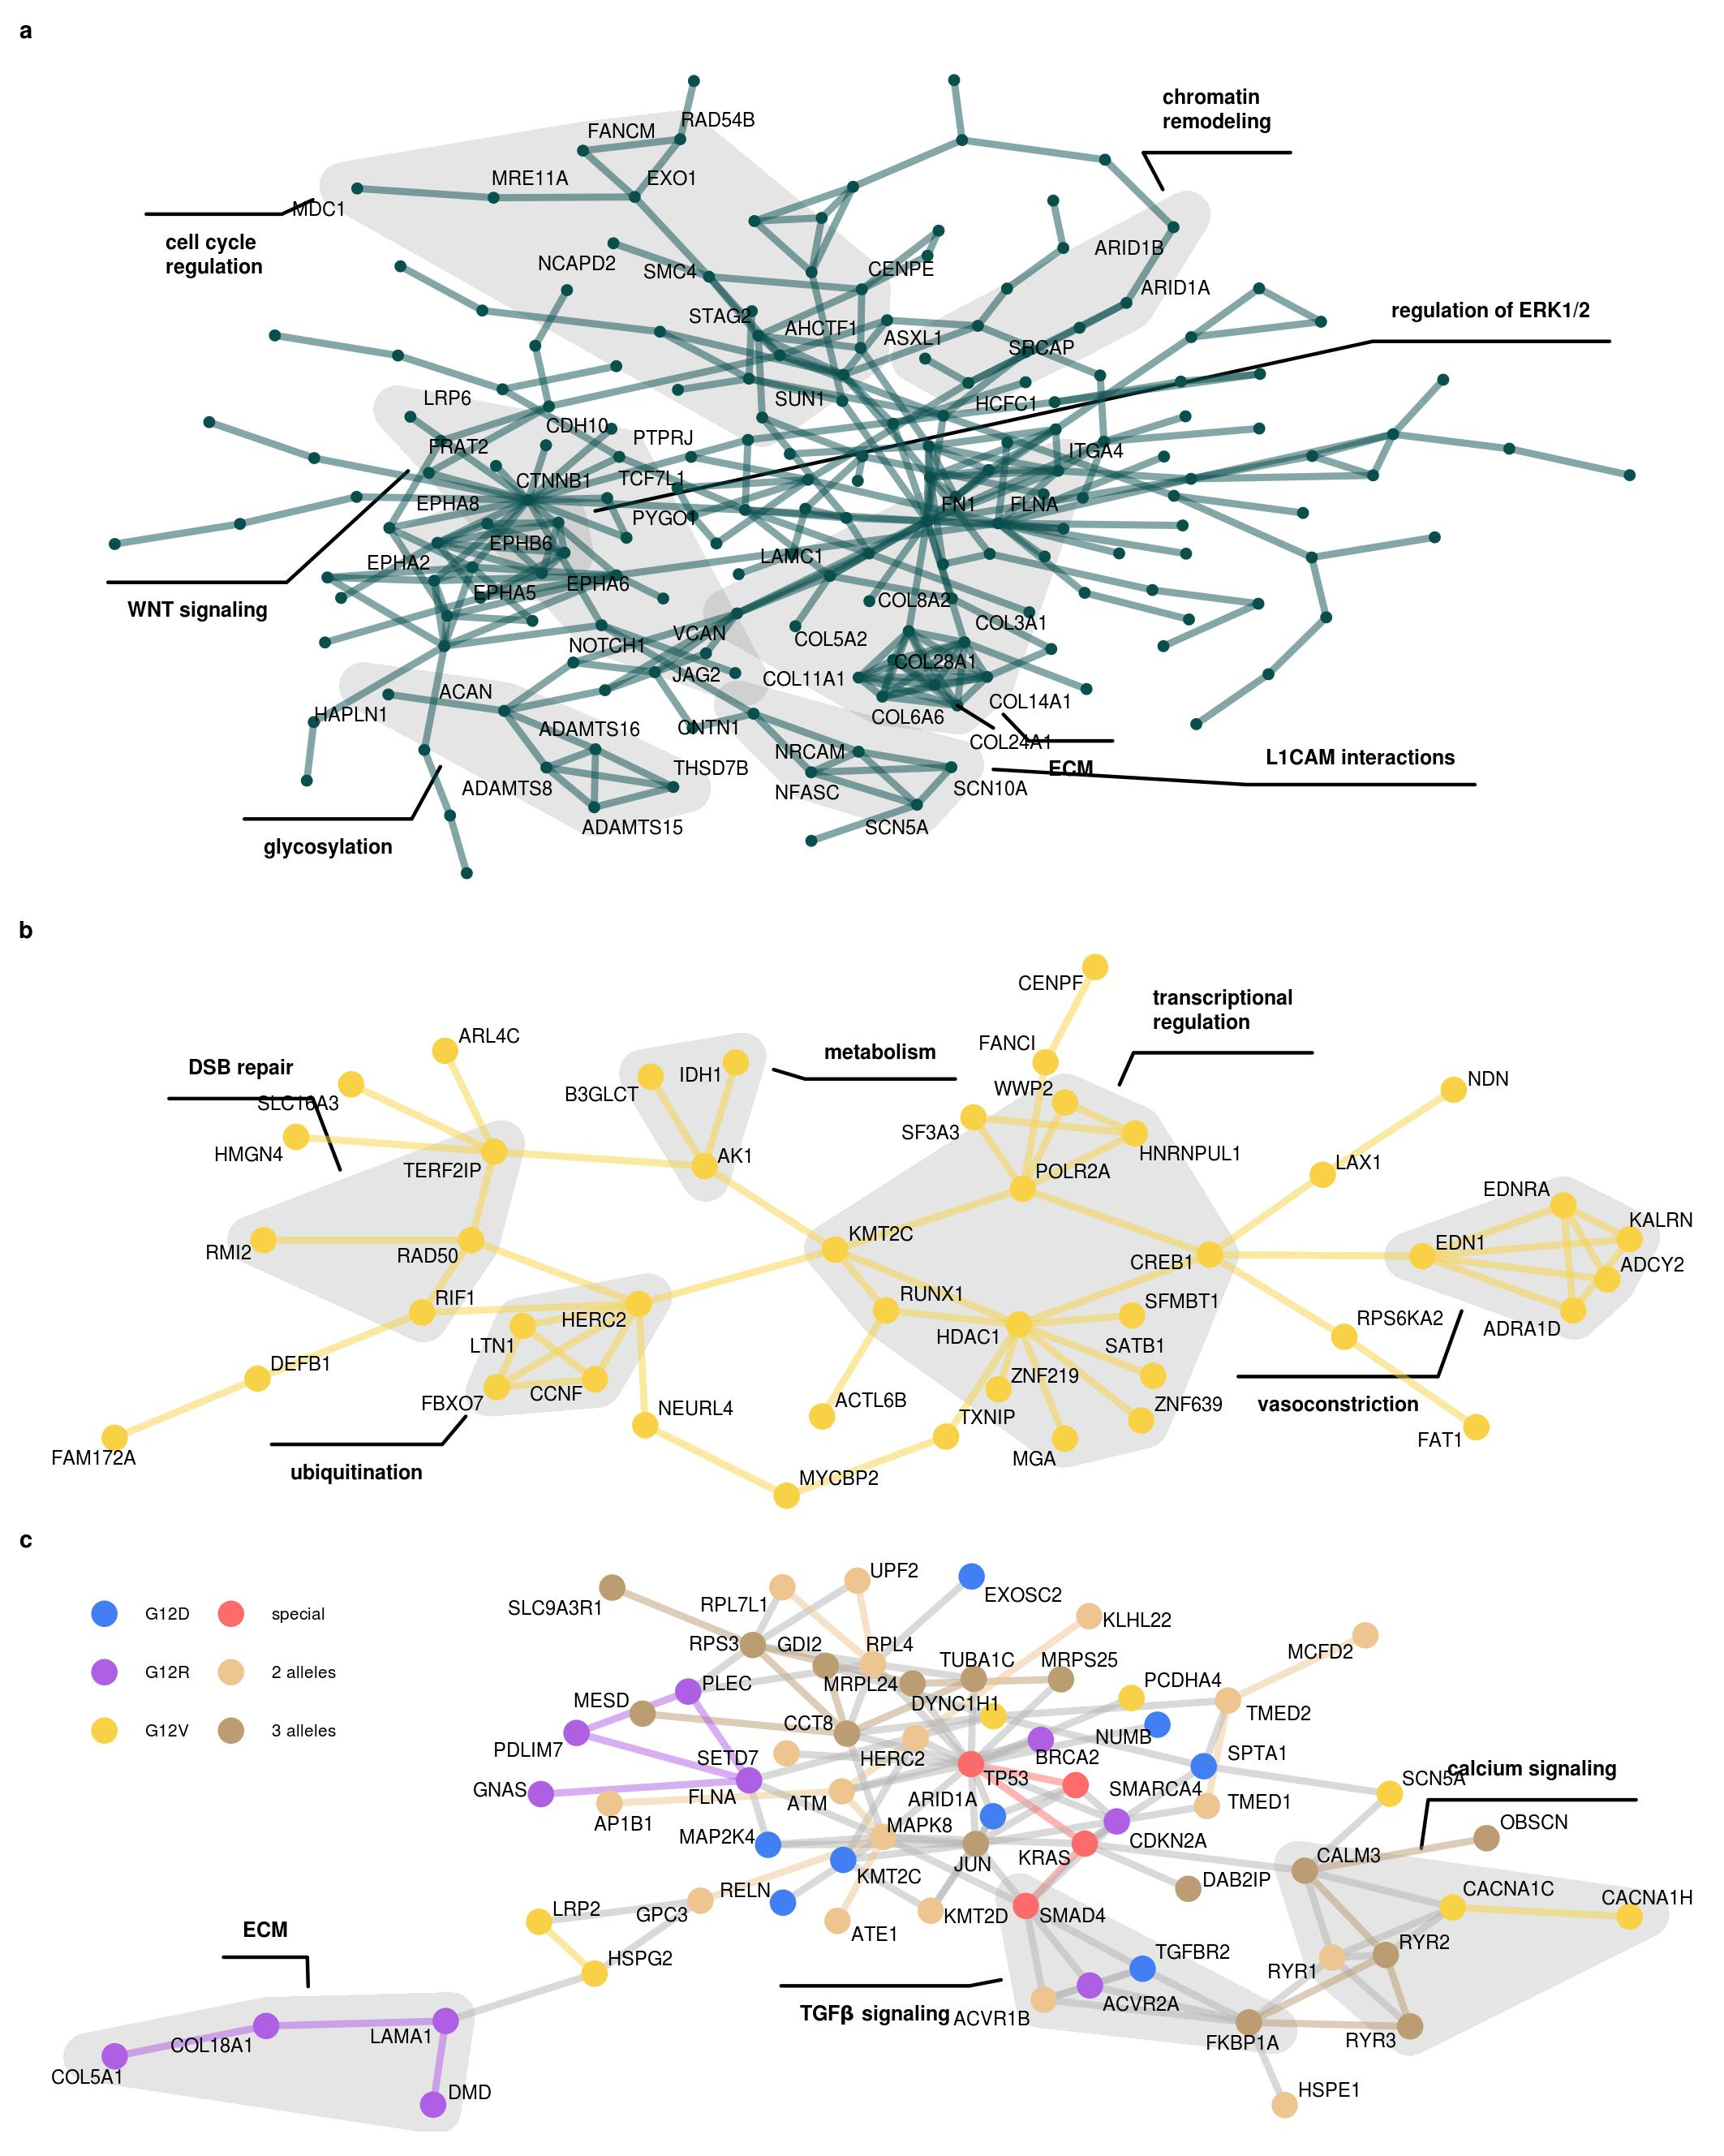
\includegraphics[width=88mm]{figures/Supp_Fig_8.jpeg}
\caption{
    \textbf{Individual genes with differential genetic dependency by \KRAS{} allele in PAAD cell lines.}
    \textbf{a.} Clustered heatmaps of the genes that demonstrated differential genetic dependency amongst cell lines of different \KRAS{} alleles in PAAD cell lines. Each column is a cell line labeled by its DepMap ID and each row is a gene.
    \textbf{b.} Examples of genes that demonstrated differential genetic dependency amongst cell lines of different \KRAS{} alleles in PAAD (*: p < 0.05, **: p < 0.01, ***: p < 0.001; p-values were adjusted using the Benjamini-Hochberg FDR correction method).
}
\label{sfig:paad-dependency-heatmap}
\end{figure}
\newpage


\begin{figure}[h!]
\centering
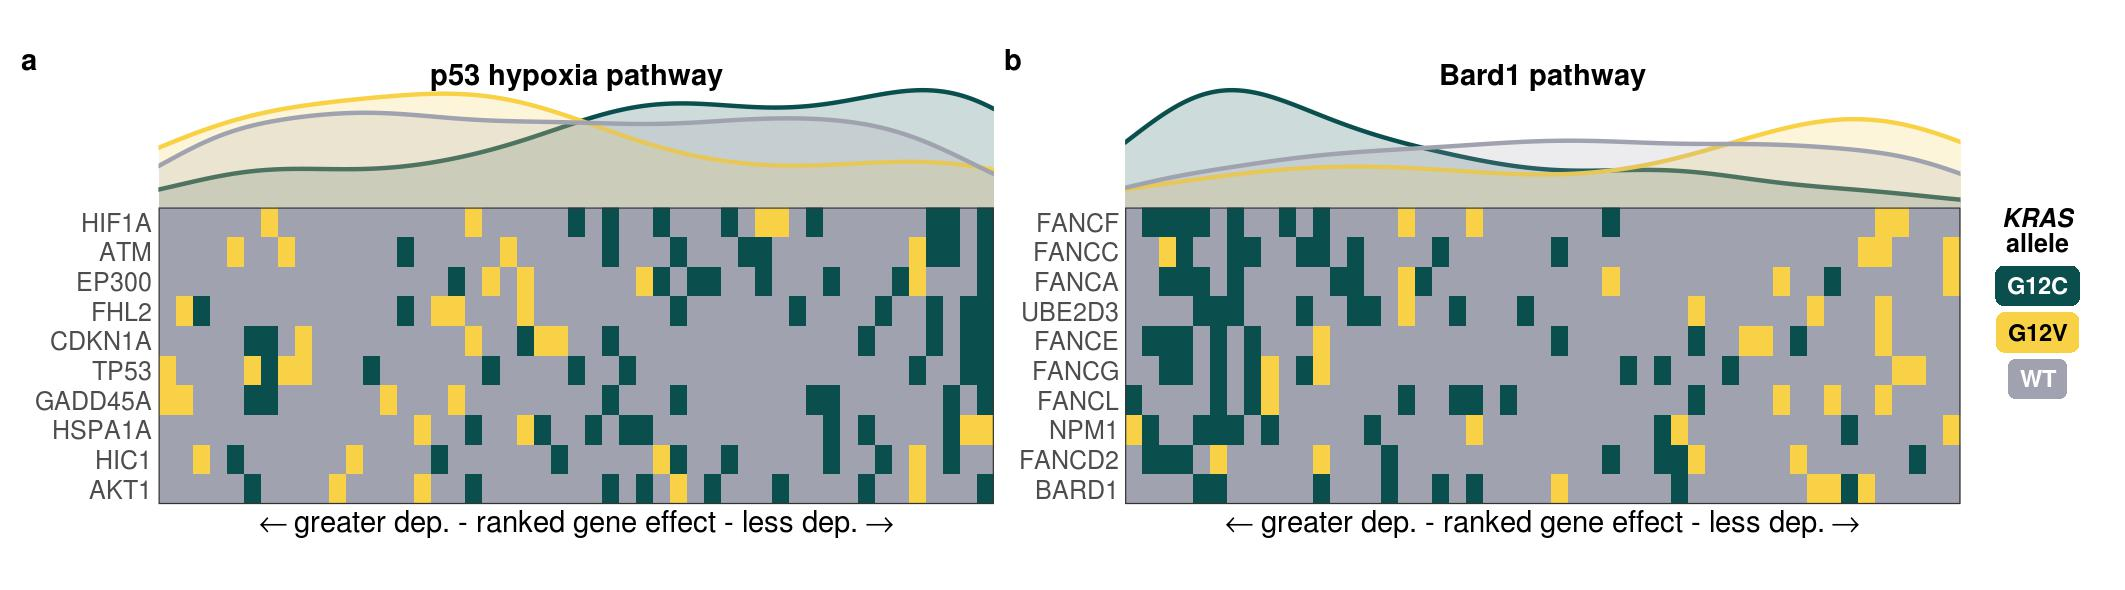
\includegraphics[width=180mm]{figures/Supp_Fig_9.jpeg}
\caption{
    \textbf{Reduced dependency on JNK signaling in PAAD cell lines with \KRAS{} G12V mutations.}
    \textbf{a.} The "JNK phosphorylation and activation by activated TAK1" gene set was significantly enriched for reduced genetic dependency in PAAD cell lines with \KRAS{} G12V. Each row represents a gene and each cell represents a cell line colored by its \KRAS{} allele. The cell lines were arranged in ranking order by their dependency score for each gene. Thus, each column indicates a rank. The line plots above the heatmap indicate the representation (density) of each \KRAS{} allele at each rank across the genes.
    \textbf{b.} The genetic dependency on \emph{MAPK8} of cell lines of different \KRAS{} alleles in PAAD (**: p < 0.01; p-values were adjusted using the Benjamini-Hochberg FDR correction method).
    \textbf{c.} The genetic dependency on \emph{JUN} and \emph{MAPK8} of cell lines of different \KRAS{} alleles in PAAD. Each point is a cell line colored according to its \KRAS{} allele. The dashed line represents the line-of-best fit. The equation, p-value, and $R^2$ for the line are shown in the top-right.
}
\label{sfig:paad-dependency-JUN}
\end{figure}
\newpage


\begin{figure}[h!]
\centering
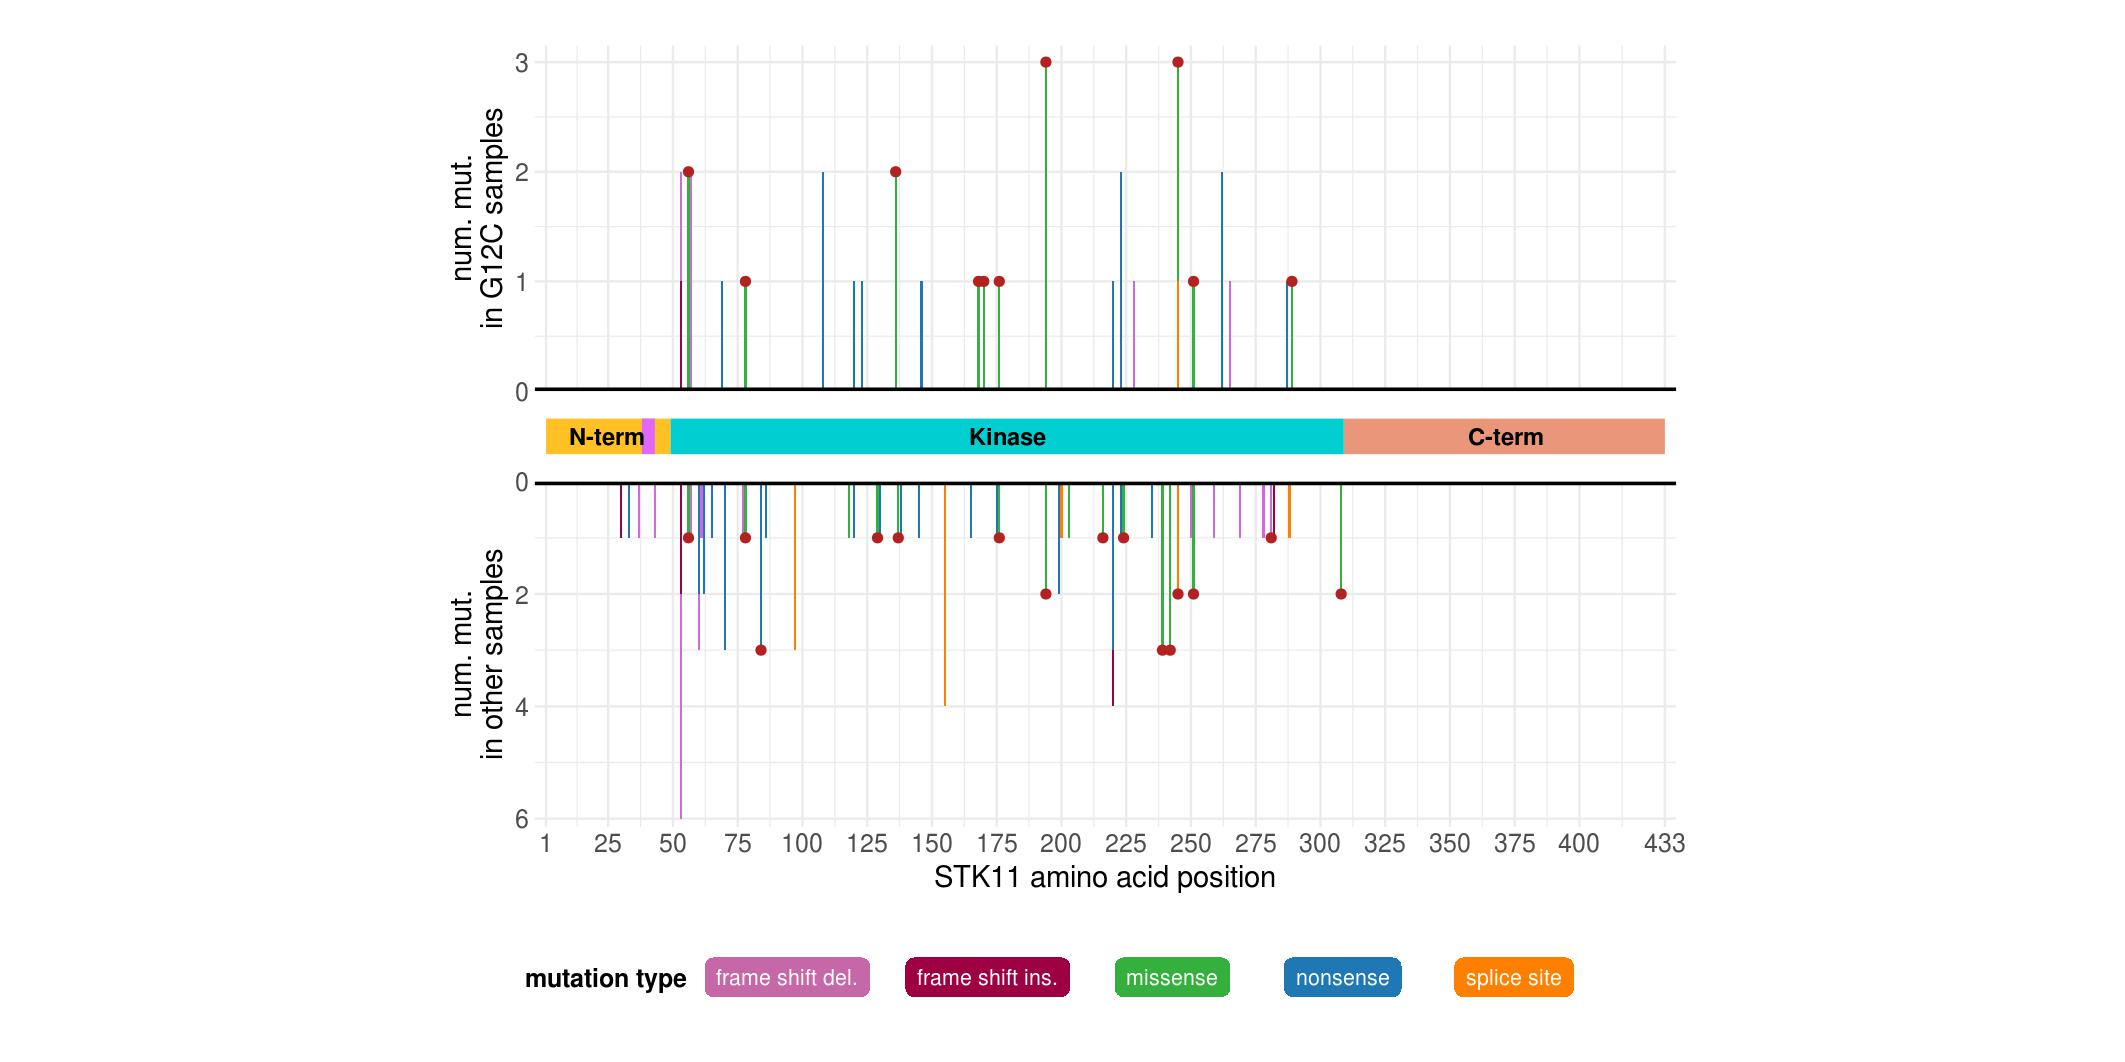
\includegraphics[width=180mm]{figures/Supp_Fig_10.jpeg}
\caption{
    \textbf{The protein modifications to STK11 in LUAD.}
    The mutations along STK11 separated by those in \KRAS{} G12C-mutant samples (top) and the rest of the samples (bottom). The color of the vertical bars indicates the type of mutation, and a red dot at the top indicates if missense mutations at the location are predicted or known to be functionally damaging. The domains of STK11 are shown between the bar-plots. The magenta portion of the N-terminus is the nuclear localization signal.
}
\label{sfig:stk11-mutation-lollipop}
\end{figure}
\newpage


\begin{figure}[h!]
\centering
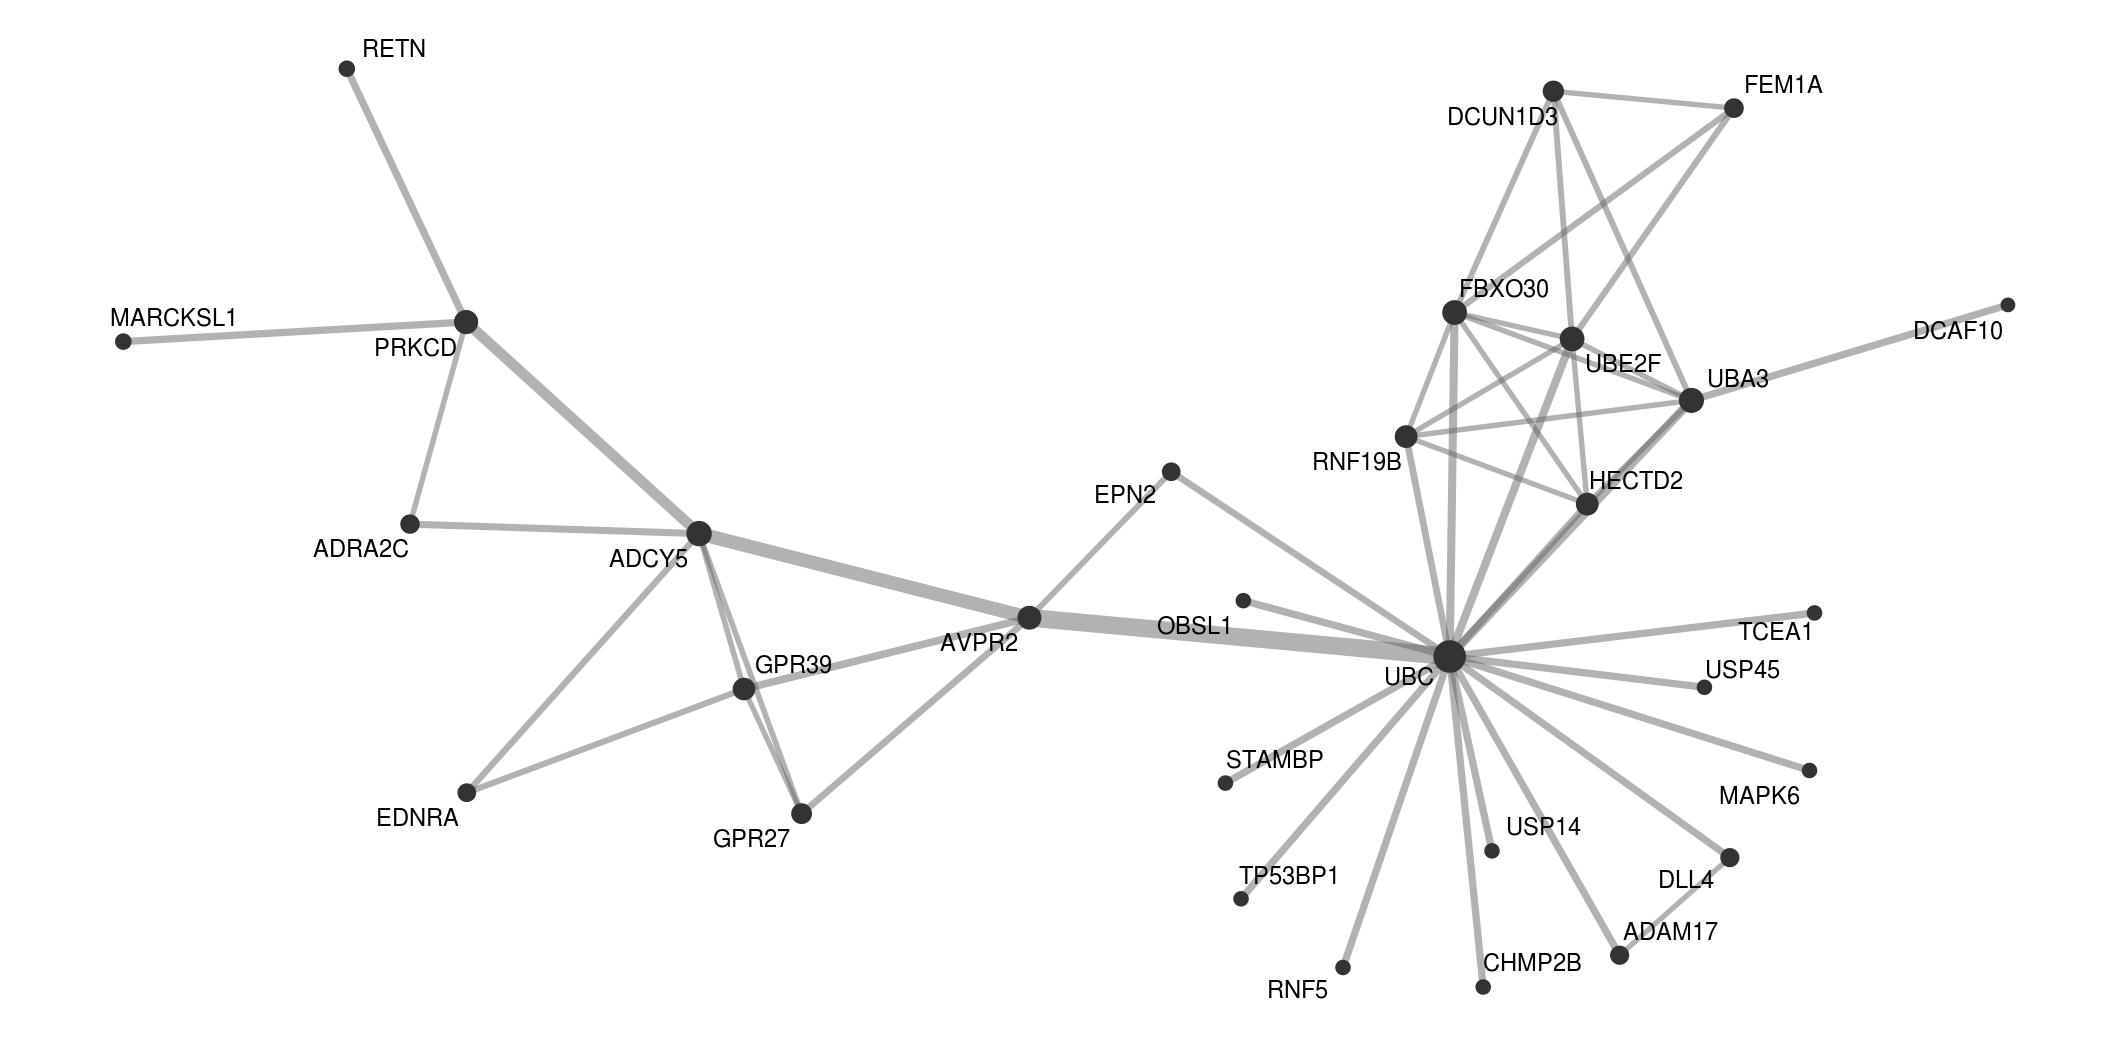
\includegraphics[width=177mm]{figures/Supp_Fig_11.jpeg}
\caption{PPIN subnetworks from the integration of comutation and genetic dependency results for \KRAS{} G12C in LUAD.}
\label{sfig:luad-integrated-ppin}
\end{figure}
\newpage

\newpage
\noindent \textbf{Supplementary Figure 11. PPIN subnetworks from the integration of comutation and genetic dependency results for \KRAS{} G12C and G12V in LUAD.}
The largest connected subnetworks of the PPIN of genes found to comutate or demonstrate differential dependence with only \KRAS{} G12C (\textbf{b}) of G12V (\textbf{b}) in LUAD were extracted. Due to the order of the G12C subnetwork, only a selection of the nodes are labeled. Curated groups of proteins with shared cellular functions are highlighted and labeled.
\newpage


\begin{figure}[h!]
\centering
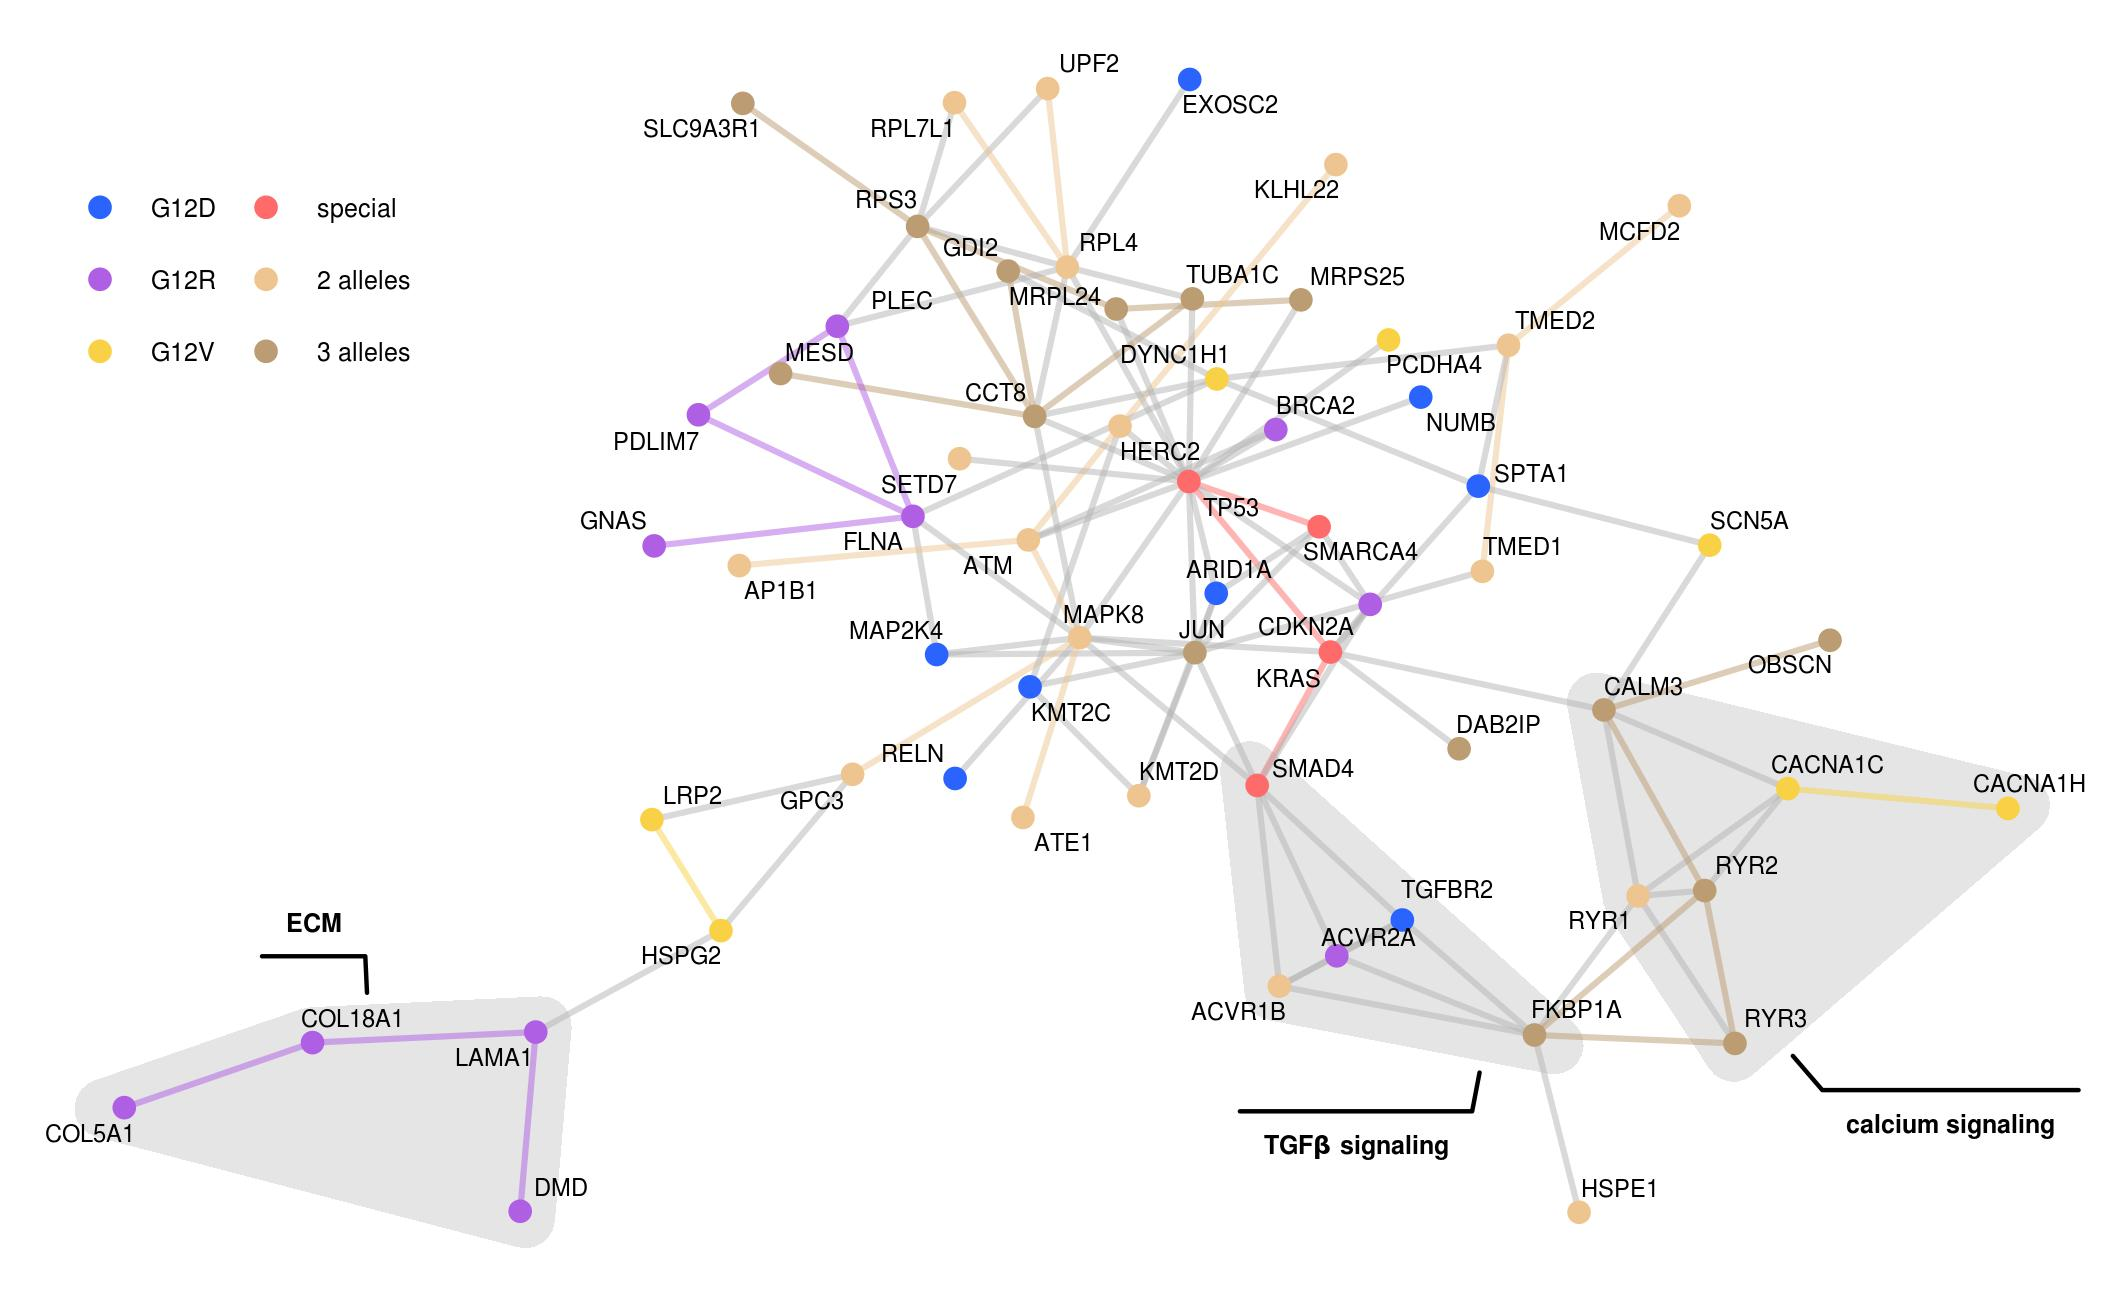
\includegraphics[width=180mm]{figures/Supp_Fig_12.jpeg}
\caption{
    \textbf{PPIN subnetworks from the integration of comutation and genetic dependency results for PAAD.}
    The largest connected subnetworks of the PPIN of genes found to comutate or demonstrate differential dependence with a \KRAS{} allele in PAAD was extracted and merged. Nodes present in multiple subnetworks are colored shades of brown, save for prominent oncogenes and tumor suppressors in COAD, shown in red ("special"). The rest of the nodes are colored by which allele they are associated with. Curated groups of proteins with shared cellular functions are highlighted and labeled.
}
\label{sfig:paad-integrated-ppin}
\end{figure}



%%TC:endignore

\end{document}
